%%%%%%%%%%%%%%%%%%%%%%%%%%%%%%%%%%%%%%%%%%%%%%%%%%%
%
%  New template code for TAMU Theses and Dissertations starting Fall 2012.  
%  For more info about this template or the 
%  TAMU LaTeX User's Group, see http://www.howdy.me/.
%
%  Author: Wendy Lynn Turner 
%
%%%%%%%%%%%%%%%%%%%%%%%%%%%%%%%%%%%%%%%%%%%%%%%%%%%

\documentclass[12pt]{report}
\usepackage[letterpaper]{geometry}
\geometry{verbose,tmargin=1.25in,bmargin=1.25in,lmargin=1.4in,rmargin=1.15in}
 \usepackage[doublespacing]{setspace}
 \usepackage{tocloft}
 \usepackage[rm, tiny,center, compact]{titlesec}
 \usepackage{indentfirst}
 \usepackage{etoolbox}
\usepackage{tocvsec2}
 \usepackage[titletoc]{appendix}
 \usepackage{appendix}
 \usepackage{tamuconfig}
\usepackage{rotating}


\usepackage{caption}
\usepackage{subcaption}
\usepackage{float}
\usepackage{url}
\usepackage{program}
\usepackage{algorithm}
\usepackage{algpseudocode}
\usepackage{verbatim}
% Added to fix issues with pdf searching in some versions of LaTeX
%\usepackage[T1]{fontenc}\usepackage{lmodern}
%%%%%%%%%%%%%%%%%%%%%%%%%%%%%

% Hyperref setup below.  You should be able to get away with using uncommenting just the first line.
%\usepackage[hidelinks]{hyperref}

% if \usepackage[hidelinks]{hyperref} doesn't work try this.
% \usepackage{hyperref}  % Hidelinks is an option that removes link visiability.  TAMU Thesis Offices prefers to not see the links. But often doesn't work.  
% 
% \hypersetup{
%     colorlinks=true,
%     linkcolor=black,
%     citecolor=black,
%     filecolor=black,
%     urlcolor=black,
% }
%%%%%%%  End of hyperref setup.  One of these two options should work, but my motto with hyperref is when in doubt, comment it out!
%%%%%%%%%  This hopefully fixes the problem with vertical spacing of section headings at the top of the page..  Commented out in 1.0.7
% \preto\section{%
% \ifnum\value{section}>0\addtocontents{toc}{\vskip-6pt}\fi
% }
% \preto\subsection{%
% \ifnum\value{subsection}=0\addtocontents{toc}{\vskip-6pt}\fi
% \ifnum\value{subsection}>0\addtocontents{toc}{\vskip-6pt}\fi
% } 
%%%%%%%%%%%%%%%%%%%%%%%%%%%%%%%%%%%%%%%%%%%%%%%%%%%%%%

\begin{document}

\renewcommand{\tamumanuscripttitle}{Virtualization of Non-Volatile RAM}
\renewcommand{\tamupapertype}{Thesis}
\renewcommand{\tamufullname}{Ayush Ruia}
\renewcommand{\tamudegree}{Master of Science}
\renewcommand{\tamuchairone}{A. L. N. Reddy}
% Uncomment out the next line if you have co-chairs.  You will also need to edit the titlepage.tex file.
\newcommand{\tamuchairtwo}{Ricardo Bettati}
\renewcommand{\tamumemberone}{P. R. Kumar}
%\newcommand{\tamumembertwo}{Radu Stoleru}
%\newcommand{\tamumemberthree}{Committee Member3}
\renewcommand{\tamudepthead}{Channan Singh}
\renewcommand{\tamugradmonth}{May}
\renewcommand{\tamugradyear}{2015}
\renewcommand{\tamudepartment}{Computer Engineering}
%\renewcommand\bibname{REFERENCES}

%%%%%%%%%%%%%%%%%%%%%%%%%%%%%%%%%%%%%%%%%%%%%%%%%%%
%
%  New template code for TAMU Theses and Dissertations starting Fall 2012.  
%  For more info about this template or the 
%  TAMU LaTeX User's Group, see http://www.howdy.me/.
%
%  Author: Wendy Lynn Turner 
%	 Version 1.0 
%  Last updated 8/5/2012
%
%%%%%%%%%%%%%%%%%%%%%%%%%%%%%%%%%%%%%%%%%%%%%%%%%%%

%%%%%%%%%%%%%%%%%%%%%%%%%%%%%% 
%% TITLE PAGE
%% The values get updated automatically.  Please do not make changes to this file other than adding/deleting committee members where necessary.
%%%%%%%%%%%%%%%%%%%%%%%%%%%%%%

\providecommand{\tabularnewline}{\\}



\begin{titlepage}
\begin{center}
\MakeUppercase{\tamumanuscripttitle}
\vspace{4em}

A \tamupapertype

by

\MakeUppercase{\tamufullname}

\vspace{4em}

\begin{singlespace}

Submitted to the Office of Graduate and Professional Studies of \\
Texas A\&M University \\

in partial fulfillment of the requirements for the degree of \\
\end{singlespace}

\MakeUppercase{\tamudegree}
\par\end{center}
\vspace{2em}
\begin{singlespace}
\begin{tabular}{ll}
 & \tabularnewline
& \cr
% If you have Co-Chairs comment out the 'Chair of Committee' line below and uncomment the 'Co-Chairs of Committee' line.
%Chair of Committee, & \tamuchairone\tabularnewline
Co-Chairs of Committee, & \tamuchairone\tabularnewline & \tamuchairtwo\tabularnewline
Committee Members, & \tamumemberone\tabularnewline\tabularnewline
% & \tamumembertwo\tabularnewline
% & \tamumemberthree\tabularnewline
Head of Department, & \tamudepthead\tabularnewline

\end{tabular}
\end{singlespace}
\vspace{3em}

\begin{center}
\tamugradmonth \hspace{2pt} \tamugradyear

\vspace{3em}

Major Subject: \tamudepartment \par
\vspace{3em}
Copyright \tamugradyear \hspace{.5em}\tamufullname 
\par\end{center}
\end{titlepage}
\pagebreak{}




 % This is simply a file that formats and adds your titlepage, please do not edit this unless you have a specific need. .
%%%%%%%%%%%%%%%%%%%%%%%%%%%%%%%%%%%%%%%%%%%%%%%%%%%
%
%  New template code for TAMU Theses and Dissertations starting Fall 2012.  
%  For more info about this template or the 
%  TAMU LaTeX User's Group, see http://www.howdy.me/.
%
%  Author: Wendy Lynn Turner 
%	 Version 1.0 
%  Last updated 8/5/2012
%
%%%%%%%%%%%%%%%%%%%%%%%%%%%%%%%%%%%%%%%%%%%%%%%%%%%
%%%%%%%%%%%%%%%%%%%%%%%%%%%%%%%%%%%%%%%%%%%%%%%%%%%%%%%%%%%%%%%%%%%%%
%%                           ABSTRACT 
%%%%%%%%%%%%%%%%%%%%%%%%%%%%%%%%%%%%%%%%%%%%%%%%%%%%%%%%%%%%%%%%%%%%%

\chapter*{ABSTRACT}
\addcontentsline{toc}{chapter}{ABSTRACT} % Needs to be set to part, so the TOC doesnt add 'CHAPTER ' prefix in the TOC.

\pagestyle{plain} % No headers, just page numbers
\pagenumbering{roman} % Roman numerals
\setcounter{page}{2}

\indent 
Virtualization  technology is powering today's cloud industry. Virtualization inserts a software layer, the hypervisor, below the  Operating System, to manage multiple OS environments simultaneously. Offering numerous benefits such as fault isolation, load balancing, faster server provisioning, etc., virtualization occupies a dominant position, especially in IT infrastructure in datacenters. Memory management is one of the core components of a hypervisor. Current implementations assume the underlying memory technology to be homogenous and volatile. However, with the emergence of NVRAM in the form of Storage Class Memory, this assumption remains no longer valid. New motherboard architectures will support several different memory classes each with distinct properties and characteristics. The hypervisor has to recognize, manage, and expose them separately to the different virtual machines. This study focusses on building a separate memory management module for Non-Volatile RAM in Xen hypervisor. We  show that it can be efficiently implemented with few code changes and minimal runtime performance overhead.

%%%%%%%%%%%%%%%%%%%%%%%%%%%%%%%%%%%%%%%%%%%%%%%%%%%
%
%  New template code for TAMU Theses and Dissertations starting Fall 2012.  
%  For more info about this template or the 
%  TAMU LaTeX User's Group, see http://www.howdy.me/.
%
%  Author: Wendy Lynn Turner 
%	 Version 1.0 
%  Last updated 8/5/2012
%
%%%%%%%%%%%%%%%%%%%%%%%%%%%%%%%%%%%%%%%%%%%%%%%%%%%

%%%%%%%%%%%%%%%%%%%%%%%%%%%%%%%%%%%%%%%%%%%%%%%%%%%%%%%%%%%%%%%%%%%%%%
%%                           DEDICATION
%%%%%%%%%%%%%%%%%%%%%%%%%%%%%%%%%%%%%%%%%%%%%%%%%%%%%%%%%%%%%%%%%%%%%
\chapter*{DEDICATION}
\addcontentsline{toc}{chapter}{DEDICATION}  % Needs to be set to part, so the TOC doesnt add 'CHAPTER ' prefix in the TOC.



\centerline{$Dedicated\ to\ my\ family.$}


\pagebreak{}

%%%%%%%%%%%%%%%%%%%%%%%%%%%%%%%%%%%%%%%%%%%%%%%%%%%
%
%  New template code for TAMU Theses and Dissertations starting Fall 2012.  
%  For more info about this template or the 
%  TAMU LaTeX User's Group, see http://www.howdy.me/.
%
%  Author: Wendy Lynn Turner 
%	 Version 1.0 
%  Last updated 8/5/2012
%
%%%%%%%%%%%%%%%%%%%%%%%%%%%%%%%%%%%%%%%%%%%%%%%%%%%


%%%%%%%%%%%%%%%%%%%%%%%%%%%%%%%%%%%%%%%%%%%%%%%%%%%%%%%%%%%%%%%%%%%%%%
%%                           ACKNOWLEDGEMENTS
%%%%%%%%%%%%%%%%%%%%%%%%%%%%%%%%%%%%%%%%%%%%%%%%%%%%%%%%%%%%%%%%%%%%%
\chapter*{ACKNOWLEDGEMENTS}
\addcontentsline{toc}{chapter}{ACKNOWLEDGEMENTS}  % Needs to be set to part, so the TOC doesnt add 'CHAPTER ' prefix in the TOC.


\indent 

I would like to express my sincere gratitude to Prof. Reddy for his guidance and support during my graduate studies. 
This project was his brainchild, and he gave me this excellent opportunity to work on it and learn, despite my past inexperience in the subject area. 
My time at Texas A\&M Univeristy has been very fruitful and enjoyable, largely due to his endless patience and compassion.
Prof. Reddy takes really good care of his students, protecting their academic as well as future professional interests, and I can never thank him enough. 

This is also an excellent opportunity to thank our academic advisor, Ms. Tammy Carda, for her countless favors extended to every student.
She has extensive knowledge of the system rules and regulations, encompassing various departments such as ISS, OGS, etc. and makes seemingly impossible tasks look easy.
On several occasions, she went out of the way to help me and sort out my troubles, when the concerned department had given up.
Be it any problem or issue concerning the life of a graduate student, when presented to her, it disappears straigtaway.
The most surprising part is that, even after helping so many students, she is always available and only an email away.
It is my good fortune to have her as an academic advisor in our department.

I would also like to thank Gim Jongmin, Viacheslav Fedorov and Allen Webb for lending their technical expertise to this project. Jongmin, especially, gave many critical feedbacks and identified several potential problems early on, resulting in a better and mature design. 

Finally, I want to thank to my parents and my brother, who have constantly provided me with guidance, love and support, my entire life. I recognize the numerous sacrifices they make everyday for my sake, and hope that I can fill their life with joy and happiness as they have done so for me.

\pagebreak{}

%%%%%%%%%%%%%%%%%%%%%%%%%%%%%%%%%%%%%%%%%%%%%%%%%%%%
%
%  New template code for TAMU Theses and Dissertations starting Fall 2012.  
%  For more info about this template or the 
%  TAMU LaTeX User's Group, see http://www.howdy.me/.
%
%  Author: Wendy Lynn Turner 
%	 Version 1.7
%  Last updated 3/24/2014
%
%%%%%%%%%%%%%%%%%%%%%%%%%%%%%%%%%%%%%%%%%%%%%%%%%%%
%%%%%%%%%%%%%%%%%%%%%%%%%%%%%%%%%%%%%%%%%%%%%%%%%%%%%%%%%%%%%%%%%%%%%%
%%       TABLE OF CONTENTS
%%%%%%%%%%%%%%%%%%%%%%%%%%%%%%%%%%%%%%%%%%%%%%%%%%%%%%%%%%%%%%%%%%%%%
% single-space sections in Table of Contents  - commented in version 1.7
%\renewcommand{\cftsecafterpnum}{\vskip0.5\baselineskip}
%\renewcommand{\cftsubsecafterpnum}{\vskip0.5\baselineskip}
%\renewcommand{\cftsubsubsecafterpnum}{\vskip0.5\baselineskip}
%%%%%%%%%%%%%%%%%%%%%%%%%%%%%%%%%%%%%%%%%%%%%%%%%%%

\phantomsection
\addcontentsline{toc}{chapter}{TABLE OF CONTENTS}  

\begin{singlespace}
\renewcommand\contentsname{\normalfont} {\centerline{TABLE OF CONTENTS}}

%\setcounter{tocdepth}{4} % This puts \subsubsection[]{×} in your List of Tables.  The default is 3.


%%%%%%%%%%%%%  Adds Page above the page number in TOC
\setlength{\cftaftertoctitleskip}{1em}
\renewcommand{\cftaftertoctitle}{%
\hfill{\normalfont {Page}\par}}



\tableofcontents

\end{singlespace}

\pagebreak{}

%%%%%%%%%%%%%%%%%%%%%%%%%%%%%%%%%%%%%%%%%%%%%%%%%%%%%%%%%%%%%%%%%%%%%%
%%                           LIST OF FIGURES
%%%%%%%%%%%%%%%%%%%%%%%%%%%%%%%%%%%%%%%%%%%%%%%%%%%%%%%%%%%%%%%%%%%%%

%commenting this portion for proposal
%\begin{comment}
\phantomsection
\addcontentsline{toc}{chapter}{LIST OF FIGURES}  

\renewcommand{\cftloftitlefont}{\center\normalfont\MakeUppercase}

\setlength{\cftbeforeloftitleskip}{-12pt} %% Positions the LOF title vertically to match the chapter titles
\renewcommand{\cftafterloftitleskip}{12pt}


\renewcommand{\cftafterloftitle}{%
\\[4em]\mbox{}\hspace{pt}FIGURE\hfill{\normalfont Page}\vskip\baselineskip}

\begingroup


\begin{center}
\begin{singlespace}
%% These values make the lof table entries appear double spaced between.
\setlength{\cftbeforechapskip}{0.4cm}
\setlength{\cftbeforesecskip}{0.30cm}
\setlength{\cftbeforesubsecskip}{0.30cm}
\setlength{\cftbeforefigskip}{0.4cm}
\setlength{\cftbeforetabskip}{0.4cm} 

%need to be worked Atin
\listoffigures

\end{singlespace}
\end{center}

\pagebreak{}

%%%%%%%%%%%%%%%%%%%%%%%%%%%%%%%%%%%%%%%%%%%%%%%%%%%%%%%%%%%%%%%%%%%%%%
%%                           lIST OF TABLES
%%%%%%%%%%%%%%%%%%%%%%%%%%%%%%%%%%%%%%%%%%%%%%%%%%%%%%%%%%%%%%%%%%%%%%
%

\phantomsection
\addcontentsline{toc}{chapter}{LIST OF TABLES}  

\renewcommand{\cftlottitlefont}{\center\normalfont\MakeUppercase}

\setlength{\cftbeforelottitleskip}{-12pt} %% Positions the LOT title vertically to match the chapter titles

\renewcommand{\cftafterlottitleskip}{12pt}


\renewcommand{\cftafterlottitle}{%
\\[4em]\mbox{}\hspace{4pt}TABLE\hfill{\normalfont Page}\vskip\baselineskip}

\begin{center}
\begin{singlespace}

%% These values make the lot table entries appear double spaced between.
\setlength{\cftbeforechapskip}{0.4cm}
\setlength{\cftbeforesecskip}{0.30cm}
\setlength{\cftbeforesubsecskip}{0.30cm}
\setlength{\cftbeforefigskip}{0.4cm}
\setlength{\cftbeforetabskip}{0.4cm}

%need to add Atin
\listoftables 

\end{singlespace}
\end{center}

\endgroup
%\end{comment}

\pagebreak{}  % Need this for the pagenumbering to be correct. 

%%%%%%%%%%%%%%%%%%%%%%%%%%%%%%%%%%%%%%%%%%%%%%%%%%%
%
%  New template code for TAMU Theses and Dissertations starting Fall 2012.  
%  For more info about this template or the 
%  TAMU LaTeX User's Group, see http://www.howdy.me/.
%
%  Author: Wendy Lynn Turner 
%	 Version 1.0 
%  Last updated 8/5/2012
%
%%%%%%%%%%%%%%%%%%%%%%%%%%%%%%%%%%%%%%%%%%%%%%%%%%%

%%%%%%%%%%%%%%%%%%%%%%%%%%%%%%%%%%%%%%%%%%%%%%%%%%%%%%%%%%%%%%%%%%%%%%
%%                           NOMENCLATURE
%%%%%%%%%%%%%%%%%%%%%%%%%%%%%%%%%%%%%%%%%%%%%%%%%%%%%%%%%%%%%%%%%%%%%

\chapter*{NOMENCLATURE}
\addcontentsline{toc}{chapter}{NOMENCLATURE}  % Needs to be set to part, so the TOC doesnt add 'CHAPTER ' prefix in the TOC.

\begin{tabular}{ll}
%IT & Information Technology \tabularnewline
IO & Input Output \tabularnewline
VMM & Virtual Machine Monitor \tabularnewline
MMIO & Memory Mapped I/O \tabularnewline
RAM & Random Access Memory \tabularnewline
NV & Non-Volatile \tabularnewline
OS & Operating System \tabularnewline
VM & Virtual Machine \tabularnewline
NVRAM & Non-Volatile RAM \tabularnewline
DIMM & Dual In-Line Memory Module \tabularnewline
SCM & Storage Class Memory \tabularnewline
API & Application Program Interface \tabularnewline
NVDIMM & Non-Volatile Dual In-Line Memory Module \tabularnewline
VA & Virtual Address \tabularnewline
PA & Physical Address \tabularnewline
%MA & Machine Address  \tabularnewline
ISA & Instruction Set Architecture \tabularnewline
%CPU & Central Processing Unit \tabularnewline
VMCS & Virtual Machine Control Structure \tabularnewline
vCPU & Virtual CPU \tabularnewline
DMA & Direct Memory Access \tabularnewline
TLB & Translation Lookaside Buffer \tabularnewline
%PCI & Peripheral Component Interconnect \tabularnewline
PCIe & Peripheral Component Interconnect Express \tabularnewline
SR-IOV & Single Root I/O Virtualization \tabularnewline
HDD & Hard Disk Drive \tabularnewline
SDD & Solid State Drive \tabularnewline
DRAM & Dynamic Random Access Memory \tabularnewline
BIOS & Basic Input/Output System \tabularnewline
ACPI & Advanced Configuration and Power Interface \tabularnewline
%VT & Virtualization Technology \tabularnewline
%AMD & Advanced Micro Devices \tabularnewline
%SVM & Secure Virtual Machine \tabularnewline
PV & Para Virtual \tabularnewline
HVM & Hardware Virtual Machine \tabularnewline
MMU & Memory Management Unit \tabularnewline
IOMMU & Input/Output Memory Management Unit \tabularnewline
%MOS & Metal Oxide Semiconductor \tabularnewline
PML4 & Page Map Level 4 \tabularnewline
GDT & Global Descriptor Table \tabularnewline
LDT & Local Descriptor Table \tabularnewline
NVM & Non-Volatile Memory \tabularnewline
ELF & Executable and Linkable Format \tabularnewline
SDK & Software Development Kit \tabularnewline
%SATA & Serial ATA \tabularnewline
IMC & Integrated Memory Controller \tabularnewline


%TxDOT \hfill{}\hfill{}\hfill{}\hfill{}\hfill{}\hfill{}\hfill{}\hfill{} & \multicolumn{1}{l}{Texas Department of Transportation}\tabularnewline
\end{tabular}

\vspace{2em}

%This page is optional.

\pagebreak{}


%%%%%%%%%%%%%%%%%%%%%%%%%%%%%%%%%%%%%%%%%%%%%%%%%%%
%
%  New template code for TAMU Theses and Dissertations starting Fall 2012.  
%  For more info about this template or the 
%  TAMU LaTeX User's Group, see http://www.howdy.me/.
%
%  Author: Wendy Lynn Turner 
%	 Version 1.7
%  Last updated 3/24/2014
%
%%%%%%%%%%%%%%%%%%%%%%%%%%%%%%%%%%%%%%%%%%%%%%%%%%%
%%%%%%%%%%%%%%%%%%%%%%%%%%%%%%%%%%%%%%%%%%%%%%%%%%%%%%%%%%%%%%%%%%%%%%
%%       TABLE OF CONTENTS
%%%%%%%%%%%%%%%%%%%%%%%%%%%%%%%%%%%%%%%%%%%%%%%%%%%%%%%%%%%%%%%%%%%%%
% single-space sections in Table of Contents  - commented in version 1.7
%\renewcommand{\cftsecafterpnum}{\vskip0.5\baselineskip}
%\renewcommand{\cftsubsecafterpnum}{\vskip0.5\baselineskip}
%\renewcommand{\cftsubsubsecafterpnum}{\vskip0.5\baselineskip}
%%%%%%%%%%%%%%%%%%%%%%%%%%%%%%%%%%%%%%%%%%%%%%%%%%%

\phantomsection
\addcontentsline{toc}{chapter}{TABLE OF CONTENTS}  

\begin{singlespace}
\renewcommand\contentsname{\normalfont} {\centerline{TABLE OF CONTENTS}}

%\setcounter{tocdepth}{4} % This puts \subsubsection[]{×} in your List of Tables.  The default is 3.


%%%%%%%%%%%%%  Adds Page above the page number in TOC
\setlength{\cftaftertoctitleskip}{1em}
\renewcommand{\cftaftertoctitle}{%
\hfill{\normalfont {Page}\par}}



\tableofcontents

\end{singlespace}

\pagebreak{}

%%%%%%%%%%%%%%%%%%%%%%%%%%%%%%%%%%%%%%%%%%%%%%%%%%%%%%%%%%%%%%%%%%%%%%
%%                           LIST OF FIGURES
%%%%%%%%%%%%%%%%%%%%%%%%%%%%%%%%%%%%%%%%%%%%%%%%%%%%%%%%%%%%%%%%%%%%%

%commenting this portion for proposal
%\begin{comment}
\phantomsection
\addcontentsline{toc}{chapter}{LIST OF FIGURES}  

\renewcommand{\cftloftitlefont}{\center\normalfont\MakeUppercase}

\setlength{\cftbeforeloftitleskip}{-12pt} %% Positions the LOF title vertically to match the chapter titles
\renewcommand{\cftafterloftitleskip}{12pt}


\renewcommand{\cftafterloftitle}{%
\\[4em]\mbox{}\hspace{pt}FIGURE\hfill{\normalfont Page}\vskip\baselineskip}

\begingroup


\begin{center}
\begin{singlespace}
%% These values make the lof table entries appear double spaced between.
\setlength{\cftbeforechapskip}{0.4cm}
\setlength{\cftbeforesecskip}{0.30cm}
\setlength{\cftbeforesubsecskip}{0.30cm}
\setlength{\cftbeforefigskip}{0.4cm}
\setlength{\cftbeforetabskip}{0.4cm} 

%need to be worked Atin
\listoffigures

\end{singlespace}
\end{center}

\pagebreak{}

%%%%%%%%%%%%%%%%%%%%%%%%%%%%%%%%%%%%%%%%%%%%%%%%%%%%%%%%%%%%%%%%%%%%%%
%%                           lIST OF TABLES
%%%%%%%%%%%%%%%%%%%%%%%%%%%%%%%%%%%%%%%%%%%%%%%%%%%%%%%%%%%%%%%%%%%%%%
%

\phantomsection
\addcontentsline{toc}{chapter}{LIST OF TABLES}  

\renewcommand{\cftlottitlefont}{\center\normalfont\MakeUppercase}

\setlength{\cftbeforelottitleskip}{-12pt} %% Positions the LOT title vertically to match the chapter titles

\renewcommand{\cftafterlottitleskip}{12pt}


\renewcommand{\cftafterlottitle}{%
\\[4em]\mbox{}\hspace{4pt}TABLE\hfill{\normalfont Page}\vskip\baselineskip}

\begin{center}
\begin{singlespace}

%% These values make the lot table entries appear double spaced between.
\setlength{\cftbeforechapskip}{0.4cm}
\setlength{\cftbeforesecskip}{0.30cm}
\setlength{\cftbeforesubsecskip}{0.30cm}
\setlength{\cftbeforefigskip}{0.4cm}
\setlength{\cftbeforetabskip}{0.4cm}

%need to add Atin
\listoftables 

\end{singlespace}
\end{center}

\endgroup
%\end{comment}

\pagebreak{}  % Need this for the pagenumbering to be correct. 
  % This is simply a file that formats and adds your toc, lof, and lot, please do not edit this unless you have a specific need. .

%%%%%%%%%%%%%%%%%%%%%%%%%%%%%%%%%%%%%%%%%%%%%%%%%%%
%
%  New template code for TAMU Theses and Dissertations starting Fall 2012.  
%  For more info about this template or the 
%  TAMU LaTeX User's Group, see http://www.howdy.me/.
%
%  Author: Wendy Lynn Turner 
%	 Version 1.0 
%  Last updated 8/5/2012
%
%%%%%%%%%%%%%%%%%%%%%%%%%%%%%%%%%%%%%%%%%%%%%%%%%%%

%%%%%%%%%%%%%%%%%%%%%%%%%%%%%%%%%%%%%%%%%%%%%%%%%%%%%%%%%%%%%%%%%%%%%%
%%                           SECTION I
%%%%%%%%%%%%%%%%%%%%%%%%%%%%%%%%%%%%%%%%%%%%%%%%%%%%%%%%%%%%%%%%%%%%%


\pagestyle{plain} % No headers, just page numbers
\pagenumbering{arabic} % Arabic numerals
\setcounter{page}{1}


\chapter{\uppercase {Introduction}}

\section{Motivation}
Proliferation of smartphones and tablets is introducing a divide in the computer industry. While mobile technology is burgeoning in the role of access points, computationally intensive tasks are being offloaded to the cloud. As a result, the server industry is growing at a tremendous pace. This has also led to the development of associated technologies, the most prominent being virtualization. 


Virtualization enables multiple Operating System environments to run simultaneously on one hardware platform. It provides added security and isolation in the form of an additional software layer below the OS, called the hypervisor. This technology has become the de-facto industry standard for large server farms. Fault Isolation, centralized control, workload balance, and live migration of machines are few of its many benefits [Provide a reference]. Hypervisors are rapidly evolving to minimize the performance penalty of the extra layer of software. 


It may seem counterintuitive, but most virtualized systems today, are constrained by memory and I/O, with ample CPU resources to spare [Provide a reference]. However, these limitations will no longer remain relevant with the upcoming radical changes in memory technologies. In the past few decades, memory subsystem structure has been fairly consistent, with revisions just in terms of size. However, new developments such as 3D memory stack, Storage Class Memory, etc., will completely revolutionize future memory architectures. 


Among these new technologies, emergence of Non-Volatile RAM in the form of SCM, has the potential to provide new opportunities in utilizing memory in to virtual machines. SCM can potentially  reduce the frequency of disk I/O operations, and free memory off disk caches, thus impacting both the constraints at the same time. No matter, the direction of future memory systems, it is likely  that persistent memory will play a dominant role in future server farms. Thus, it is a natural and worthwhile initiative to inspect the possibility of sharing such a resource in Virtual Machines, with immense scope for  performance gains in filesystems, boot procedure, crash recovery, etc [ref]. This  thesis is going to focus on some of these aspects. To the best of our  knowledge, there has been no prior work in this direction, and this work can be considered as a first step in enabling NVRAM sharing in virtualized environments

\section{Virtualization}
Modern day computers are a combination of extremely complex software and hardware systems. Such a high level of engineering is made possible through concepts of abstraction, where an upper layer interacts with the layer beneath it, using well defined interfaces, oblivious to its inner implementation complexity and details.

A computer system can be viewed as a stack of several independent layers as shown in Fig~\ref{fig:appstack}. Here the flexibility of each layer is constrained by the interfaces defined both above and below it. 

\setlength{\belowcaptionskip}{-10pt}

\begin{figure}[H]
  \centering
  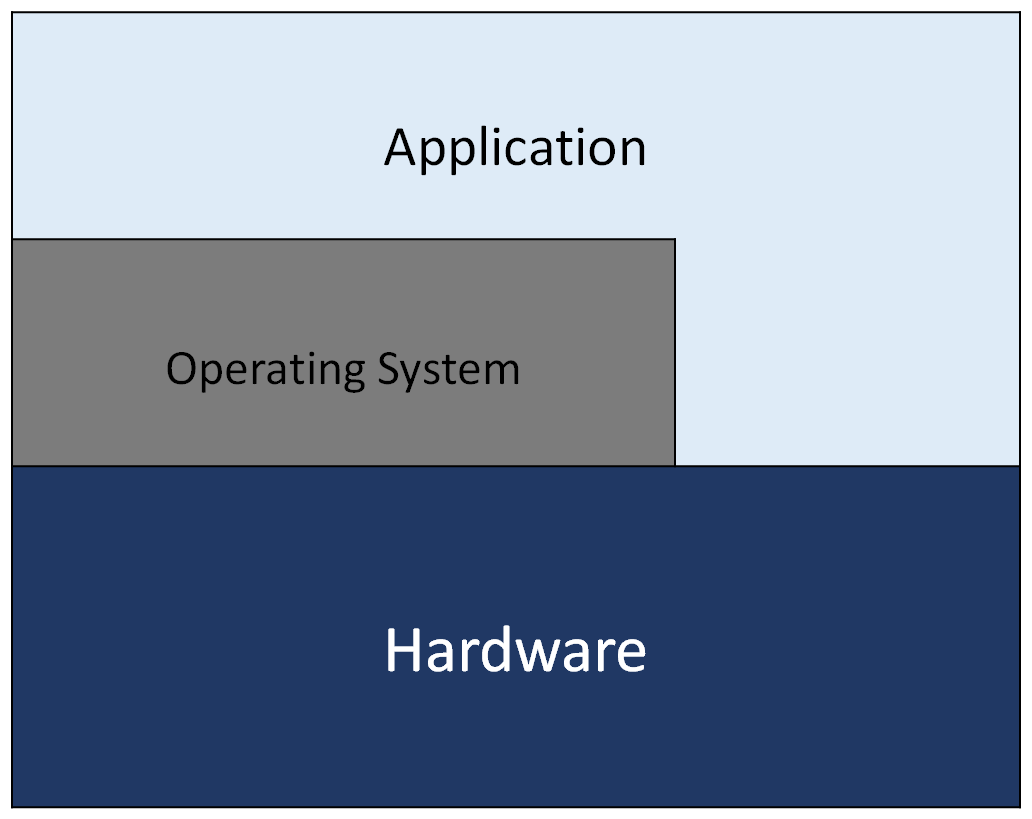
\includegraphics[scale=0.6]{figures/app_stack.png}
  \caption{Conventional Application Stack}
  \label{fig:appstack}
\end{figure}

Virtualization provides a way to relax the above constraints, either in the form of the entire system or a subsystem like memory, I/O processor etc. It enables the mapping of a virtual system, to real system resources thereby giving an illusion to the process/OS of a custom virtual environment, different from the host machine.

Formally, virtualization can be defined as a mapping between a guest state ($S_i$) and a host state ($S'_i$), such that a sequence of operators, $e_k$, modifying the guest state from ($S_i$) to ($S_j$), can be represented by some corresponding sequence of operators, $e'_k$, which modifies the host state from ($S'_i$) to ($S'_j$) respectively. 

\setlength{\belowcaptionskip}{-10pt}

\begin{figure}[H]
  \centering
  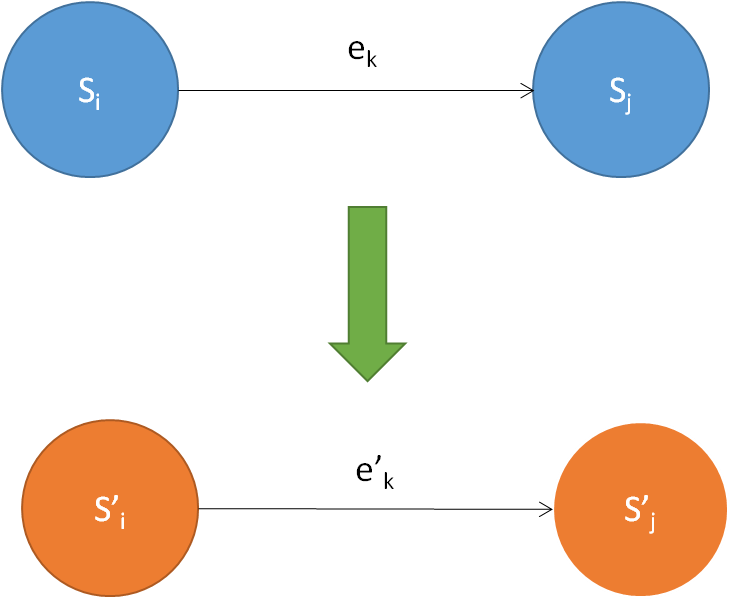
\includegraphics[scale=0.6]{figures/vir_phy_map.png}
  \caption{Equivalent State Mapping}
  \label{fig:statemap}
\end{figure}

In this work all further references to virtualization would be from the perspective of decoupling the Operating System from the actual machine configuration, and enable sharing of the resources with different VMs’ in a concurrent manner. From an OS's point of view, all hardware can be classified into three broad categories. 

1. CPU: A CPU is a highly complex piece of hardware abstracted for the OS in the form of an Instruction Set Architecture. The ISA defines the actual hardware software interface in a machine, converting software code into electrical signals which percolate through the entire system. Every action performed by the software stack (including controlling Memory and I/O) takes place through the available set of ISA instructions. 

2. Memory: Memory is just a collection of byte addressable registers which can be used to store and retrieve data. Each of these registers do not have any special functionality, only serving the purpose of data storage. Every ISA provides special instructions to interact with memory. 

3. I/O: All devices apart from CPU and Memory, such as modem, printer, monitor, etc., come under the category of I/O devices. These devices are essentially composed of several specialized registers which can be programmed to perform device specific instructions. Thus from the CPU’sperspective, there is not much of a difference between I/O and memory, since both are collection of byte addressable memory elements. Interactions with an I/O device can be performed by either (optional) special I/O instructions or standard memory instructions supported by the ISA. Due to the vast variety of devices available from different manufacturers, individual device drivers have to be developed and added to the OS separately. 


\setlength{\belowcaptionskip}{-10pt}

\begin{figure}[H]
  \centering
  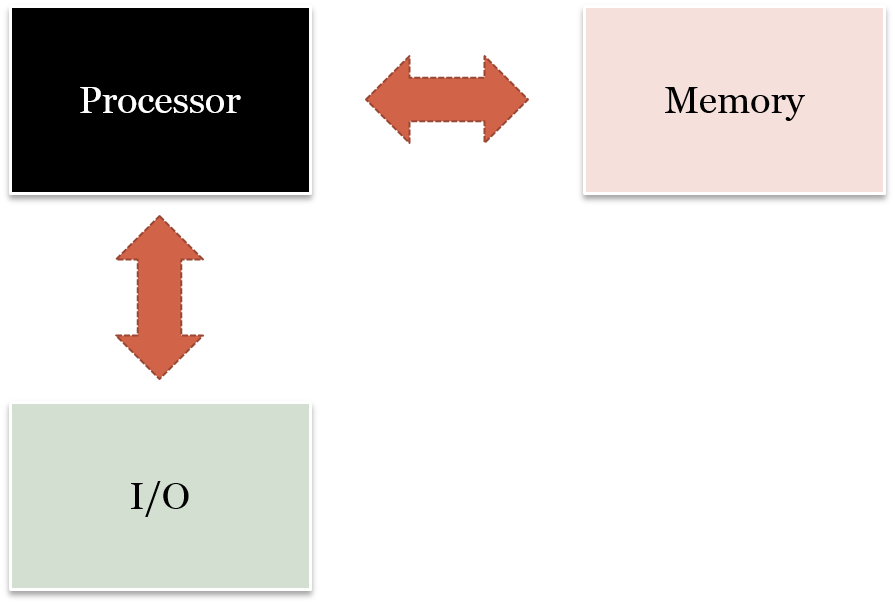
\includegraphics[scale=0.6]{figures/Mem_IO_CPU.png}
  \caption{Abstract Computer Model}
  \label{fig:mem_io}
\end{figure}

For entire system virtualization, we have to virtualize all the subsystems. This can be performed either in software, or by hardware. A software approach provides higher flexibility at the cost of reduced performance when  compared to a hardware solution. We further go into each specific subsystem virtualization specifics: 


\subsection{CPU Virtualization}

The main objective here is to give an illusion to each VM of pseudo machines, while maintaining control of the actual hardware resources at the hypervisor. Work of similar nature is performed at the application layer by the Operating System. To facilitate such protection mechanisms, a typical ISA implements several privilege levels (protection rings), allowing a certain class of instructions to execute only in a privileged mode. The ISA generally presents two levels -- user level and supervisor level. An attempt to execute a privileged instruction in an unprivileged mode triggers an exception. It transfers control of execution to a specific supervisor level subroutine (generally registered with the OS), which takes appropriate action maintaining the security and protection of the system. 



\setlength{\belowcaptionskip}{-10pt}

\begin{figure}[H]
  \centering
  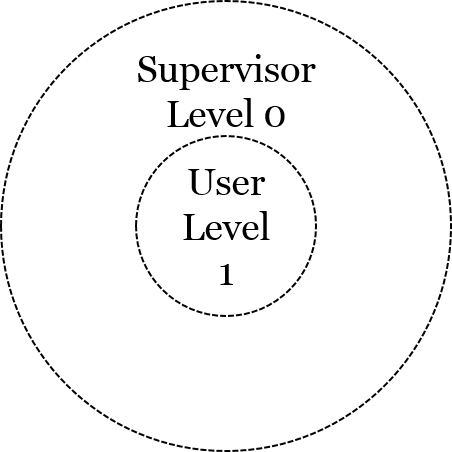
\includegraphics[scale=0.6]{figures/protect_levels.png}
  \caption{ISA Protection Rings}
  \label{fig:protect_2}
\end{figure}

In the case of virtual machines, such a task becomes all the more challenging, as these protection mechanisms have to be implemented at the OS level, by the hypervisor. Pioneering work done by Popek and Goldberg, in [1], defined several constraints on the Instruction Set Architecture of the machine to provide efficient virtualization where majority of the operations run naively on the CPU ISA instructions. The CPU instructions are first classified in the following manner 

1. Privileged Instructions: The group of instructions that can only be run when the CPU is in supervisor mode, and will trap outside it. 

2. Control Sensitive Instructions: Instructions that change the hardware configuration or resources of the system. 

3. Behavior Sensitive Instructions: Any instruction, whose output depends upon the current state, or configuration of the machine. 

 
They proposed that for any architecture to be efficiently virtualizable, all sensitive (behavior and control) instructions must be privileged instructions. Any instruction, which either tries to modify hardware configuration, or whose output depends upon it, should transfer control of execution to the hypervisor.

Contrary to norm, an operating system on a VM runs in de-privileged user mode. Most of the operations run at native speeds without emulation, with a penalty introduced only for sensitive instructions which trap into the hypervisor. 

\setlength{\belowcaptionskip}{-10pt}

\begin{figure}[H]
  \centering
  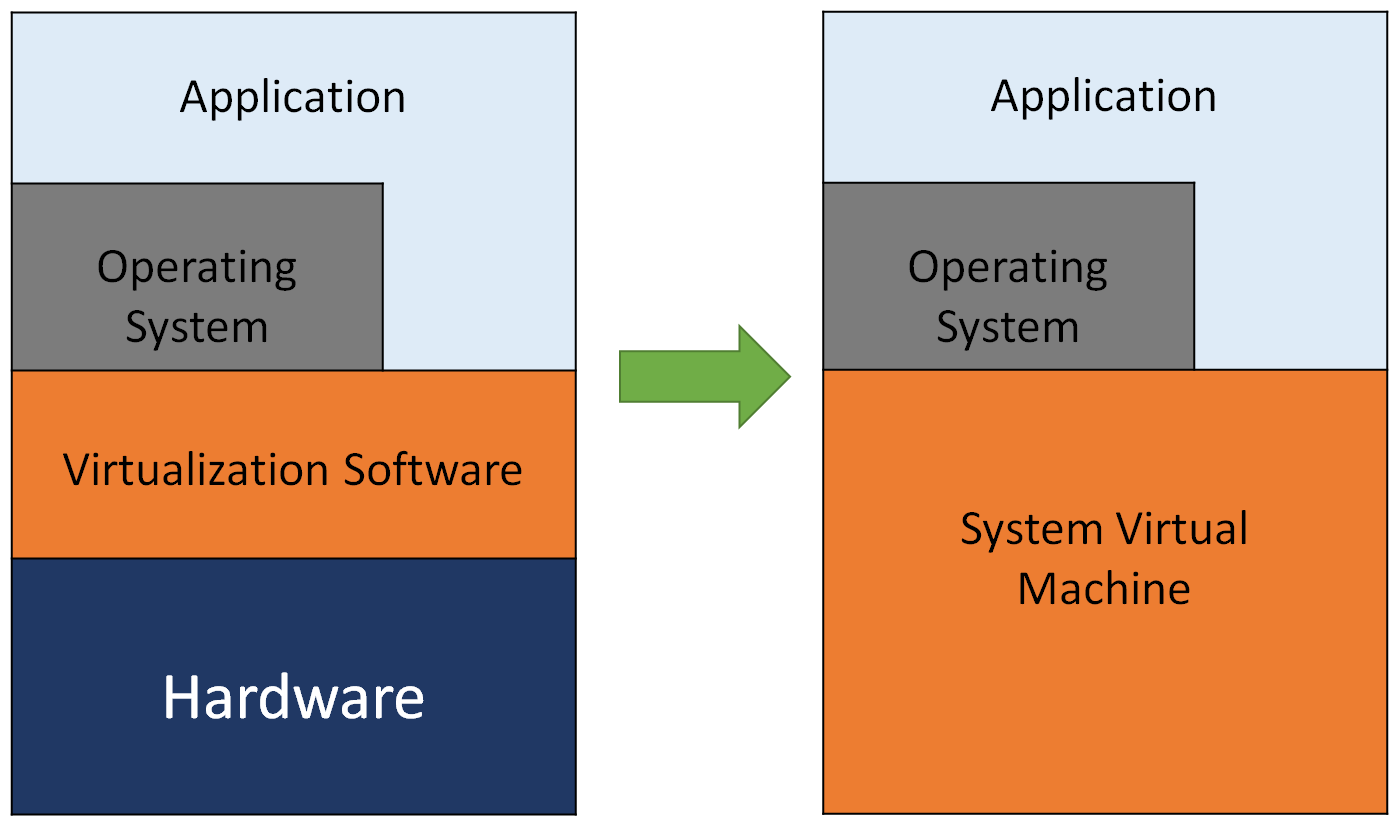
\includegraphics[scale=0.6]{figures/sys_virt.png}
  \caption{System Virtualization Model}
  \label{fig:sys_virt}
\end{figure}

According to the above definition, x86 is not a virtualizable architecture. It has a set of 17 sensitive instructions which do not trap to the supervisor mode. Being a predominant architecture in today’s computers, significant efforts have been spent producing several solutions.  

1. Emulation is the most versatile solution, implemented entirely in software. Here, the dynamic instruction stream is scanned for sensitive instructions, which are then replaced by emulated operations. Emulation can also allow a code, compiled for one ISA, to run on a host machine with a different ISA; though with a severe performance penalty (since every instruction has to be emulated). Binary translation can be viewed as an optimized version of the above, where emulated code segments are cached aggressively, providing significant performance boost for re-entrant code segments. VMWare specializes in virtualization tools with Binary Translation [ref]. 


2. Paravirtualization is another solution which relies on relaxing some of the tenets of virtualization by modifying the source code of operating system to replace sensitive operations with hypercalls to the hypervisor. Unfortunately, this trades off flexibility with performance, allowing only open source operating systems, to run on Virtual Machines. Xen is one of the leading open-source hypervisors employing paravirtualization, now natively supported by the Linux kernel (from Linux kernel 3.0 onwards). 


3. With increasing demand for virtualization technology both Intel and AMD have extended the x86 ISA to include extra features to support a hypervisor in an additional ring at -1 level. As per the original requirements of Popek and Goldberg, the OS executing in the ring 0 is oblivious to the presence of the hypervisor, with the privileged instructions generating a trap to the hypervisor. Additional level of memory virtualization is also introduced with the addition of Extended Page Tables in hardware. Along with the above, several instructions were also added to the ISA to support a system call structure for the hypervisor, named hypercalls. It includes a hardware concept of virtual CPUs with specific instructions to store/restore the state to/from VMCS. This enables x86 to achieve the status of a virtualizable architecture with the support of these extensions. Detailed explanation is provided in section Intel VT. 

\setlength{\belowcaptionskip}{-10pt}

\begin{figure}[H]
  \centering
  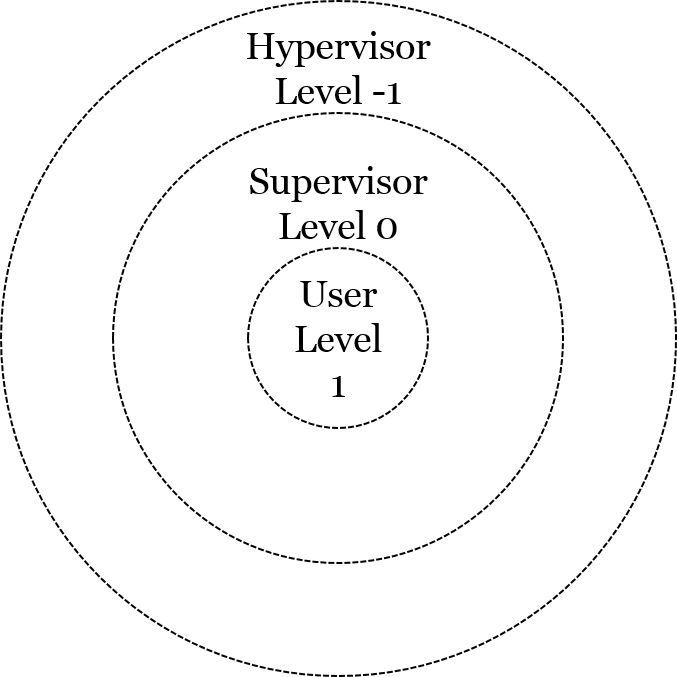
\includegraphics[scale=0.6]{figures/protect_hyper.png}
  \caption{Hypervisor Protection Rings}
  \label{fig:hyper_rings}
\end{figure}

\subsection{Memory Virtualization}
Virtual Memory has been around for a long time, allowing multiple applications to share the physical memory in the system. Each application is given a virtual address space, which is mapped on to the available physical address space via page tables maintained by the Operating System. This allows an application to be designed with respect to virtual addresses, without worrying about the runtime memory space allocation. On the downside, each memory reference now requires an address translation through the page table structure. Most ISA’s provide support for a hardware page walker which performs the translation in hardware. 


\setlength{\belowcaptionskip}{-10pt}

\begin{figure}[H]
  \centering
  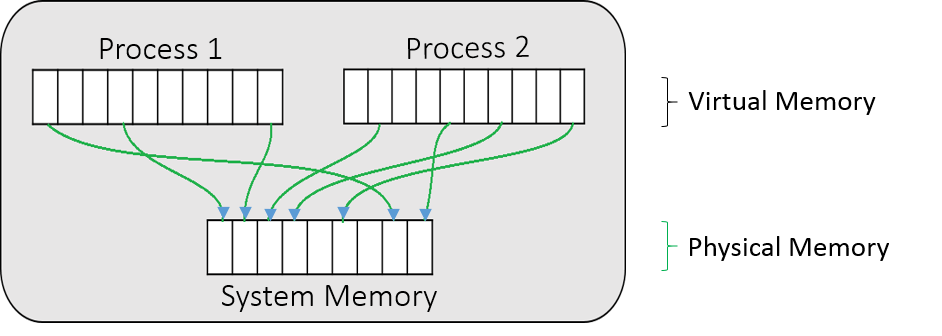
\includegraphics[scale=0.6]{figures/virt_mem.png}
  \caption{Virtual Memory}
  \label{fig:virt_mem}
\end{figure}

With respect to system level virtualization, the system memory is shared among several guest VMs. Thus it leads to an additional address space. 

1. Virtual address space: The address space as visible to applications.

2. Guest Physical address space: Individual VM level or OS level address space.

3. Real or Machine address space: The actual system memory address space. 


\setlength{\belowcaptionskip}{-10pt}

\begin{figure}[H]
  \centering
  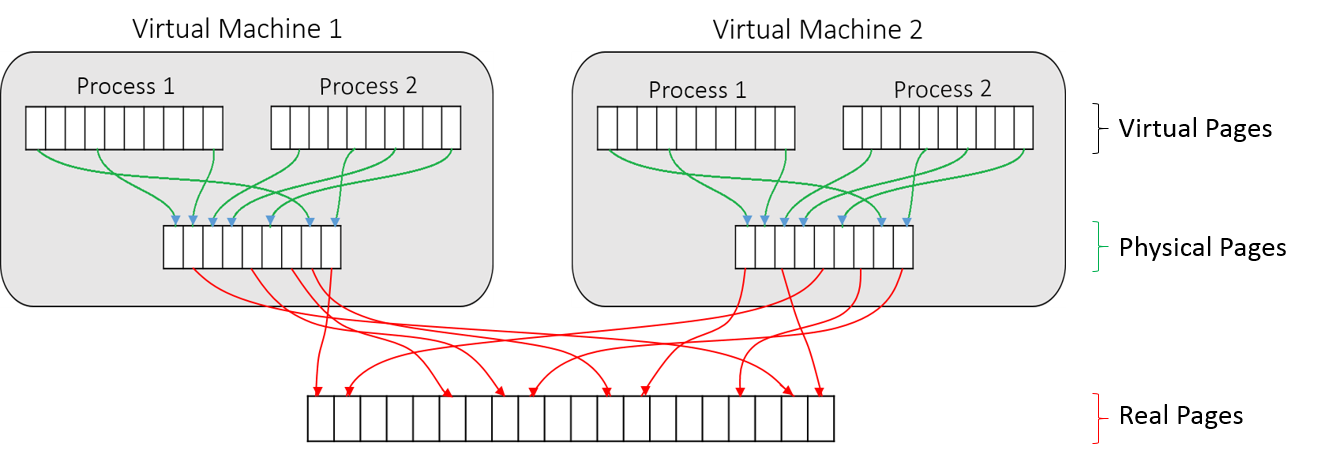
\includegraphics[scale=0.6]{figures/hyp_mem_map_comp.png}
  \caption{Hypervisor based Memory Layers}
  \label{fig:hyper_mem}
\end{figure}

Translations from virtual address space to the machine address space requires two levels of paging: 

1. Operating System Page tables: Translates from virtual to guest physical addresses.

2. Hypervisor Page tables: Translates from guest physical to machine addresses.

Without additional hardware support, a clever software based solution is to maintain an additional shadow page table with the hypervisor, mapping virtual addresses directly to machine addresses. This approach though avoids one level of paging, causes frequent traps to the hypervisor, which are very expensive. 

However, recent virtualization extensions added to the x86 architecture now support nested page tables, i.e. two levels of address translations in hardware. It provides far superior performance as compared to the shadow page table approach. In the event of a page fault due to an invalid entry in the guest page tables, the hypervisor need not be involved. However, in the software based approach, the hypervisor first catches the exception and forwards the event to the guest kernel for an appropriate response. It results in two unnecessary context switches, which can be avoided with nested page table support, where the exception is directly delivered to the guest. Moreover, any update to the guest page tables have to go through hypervisor, either via hypercalls or exceptions. As evident, the number of context switches keep multiplying for shadow page tables. On the downside, a TLB miss results is quite expensive, as the hardware has to traverse higher number of page tables to resolve an address. 

Frequent context switches is another common issue faced in virtualized systems. To reduce its impact, the virtualization extensions provide tagged TLB entries, where TLB entries are associated with a vCPU using a tag. Thus every context switch does not necessitate a complete TLB flush. It can be safely assumed from the above that hardware extensions add significant boost to most virtualized environments, especially for memory management.

\subsection{I/O Virtualization}

An I/O operation is typically controlled by programming special registers on the device, and using DMA for data transfers. Since device speeds are extremely slow (when compared to CPU) it is best not to involve the CPU. Thus DMA requests are moderated entirely by the northbridge chipset (see Fig 7). The CPU is notified of the completion of the DMA operation, using an interrupt. Device virtualization mainly focusses on the following two aspects. 

1. DMA 

2. Interrupts 

There are several ways to approach this problem. A direct method would be for the hypervisor to manage all the devices directly, and then emulate them for each Virtual Machine. It is a humungous undertaking requiring re-development of  device drivers separately for the hypervisor. An alternate and currently popular way is to assign devices to specific privileged domains, which in turn, handle the I/O requests of all the other domains. Herein arises a security issue, where DMA requests from the driver domain can corrupt memory regions of other virtual machines. Traditionally there exists no security checks in hardware to prevent devices from accessing memory regions. As a result, the VM controlling a device, can potentially gain access to the entire machine address space. 

 

Newer extensions such as VT-d (from Intel) can safeguard against such situations. VT-d implements IOMMU which act as a MMU for devices. The hypervisor can program page tables in the IOMMU mapping the device to the guest physical address space of a particular VM, maintaining memory isolation for the other guests. Moreover VT-d also includes functionality for remapping interrupts to a particular virtual CPU construct. It helps minimize costly context switches and hypervisor interventions. 

 

Newer ambitious approaches similar to PCI-e SR-IOV technology, define certain standards for devices to divide itself into smaller units. These smaller device units can then be directly controlled by individual VMs without hypervisor intervention. The hypervisor only maintains control of higher level functionality of the device, such as allocation of units to different VMs. Unfortunately, due to the vast number of devices and manufacturers involved, industry has not come to a common consensus, and the above approach is still in the nascent stages of development. 

\section{Non-Volatile Memory}

Traditionally a computer has two forms of data storage.

1. Main memory or RAM.

2. Secondary storage or Disk.

The key property of main memory is byte addressable data, while that of secondary storage is non-volatility -- data is preserved in the absence of power. Traditionally main memory has been volatile, while data on disk storage could only be accessed in blocks (~ 512 B to 4 KB). Moreover, disk is significantly slower and has enormous capacity in comparison to RAM (see Tab:~ref{tab:nvmemtable}). These factors have led RAM to serve as a level of cache for movement of data to and from disk. 

\setlength{\belowcaptionskip}{-10pt}

\begin{table}[H]
  \centering
  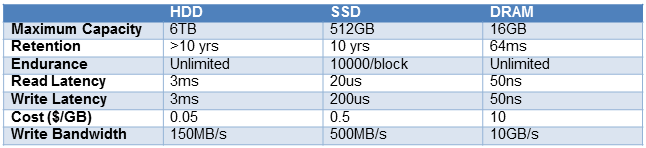
\includegraphics[scale=0.6]{figures/nvmemorytable.png}
  \caption{Comparison between HDD, SSD and DRAM (approx. values)}
  \label{tab:nvmemtable}
\end{table}

Here in, lies an issue where the volatility of RAM leads to data loss on shutdown. In the case of a planned shutdown, data residing on RAM is backed up on the disk. The system state is restored on boot up by transferring all saved data back to RAM, generating an illusion of persistence of data. However, the heart of the problem lies in the case of unplanned power failures where all data present in the main memory is permanently lost. Several different approaches can be taken to safeguard against such a situation: 

1. Software solution: -- This method cannot completely eliminate data losses, but tries to minimize the effective data loss. Here, the OS maintains complex data structures along with logging and check-pointing procedures to periodically transfer data to disk. Since disk speeds are significantly slower, heavy performance penalty is observed. The frequency of the above mentioned procedures involves a constant trade-off between performance and data integrity, where one has to be sacrificed for the other. This issue is exacerbated in server farms, where client data safety is of utmost importance. As a result, more often than not, we end up sacrificing performance. 

2. Un-interruptible power source: -- This solution comes at steep infrastructure costs of a backup power source, which lies idle for the most part.

3. Hardware solution: -- Non-volatile RAM is a proposed hardware solution to the above mentioned issues. It combines near RAM access speeds with data retentive technologies to provide performance as well as data integrity. Data movement on the memory bus is several orders of magnitude faster when compared to disk, providing persistence at little or no additional cost. 

Out of these three possibilities, the software solution is most commonly applied to current systems, due to the absence of an inexpensive alternative. Whereas, NVRAM technology, though in its nascent stages, is the most promising solution in the future systems. In conclusion, Non-Volatile memory is only useful to safeguard against data loss during unexpected power cuts. Every other usage can be served with a combination of RAM and disk (neglecting reduction boot times, as it is unimportant in virtual machines). 

\subsection{Storage Class Memory}

Research and innovation into devices have allowed a new class of memory technologies to spring up under the banner of Storage Class Memory which fall in the NVRAM category. Some common examples are PCM (Phase change memory), STT-RAM (Spin Transfer Torque RAM), ReRAM (Resistive RAM), FRAM (Ferroelectric RAM), MRAM (Magnetic RAM), etc. Each of these devices have different properties in terms of power efficiency, speed, density, and cost/bit, but are unified by the following common characteristics.

1. Byte Addressable Memory

2. Non-volatility

3. Significantly faster access times when compared to disks or SSDs.

Introduction of SCM will see a change in the motherboard architecture. As shown in Fig~\ref{fig:new_arch}, it can be placed alongside DRAM on the memory bus, and also on a PCIe bus along with SSDs. With the growth and commercialization of different SCM technologies, SCM is expected to replace/augment both DRAM and Flash memory from their dominant roles in conventional machines in the near future. 

\setlength{\belowcaptionskip}{-10pt}

\begin{figure}[H]
  \centering
  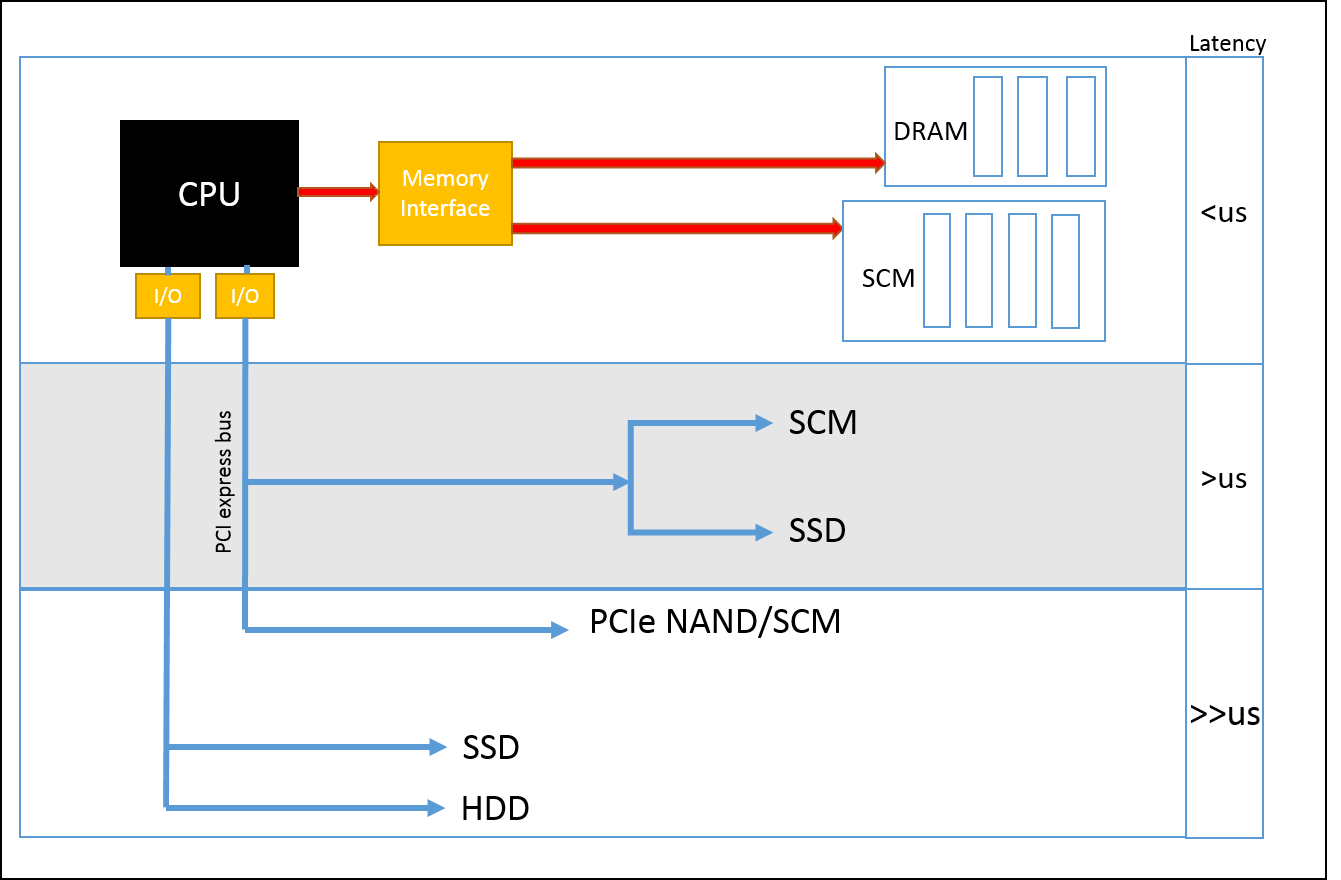
\includegraphics[scale=0.6]{figures/new_mem_arch.png}
  \caption{SCM based Motherboard Architectures}
  \label{fig:new_arch}
\end{figure}

\subsection{NVDIMM}
Meanwhile another form of Non-volatile RAM in the form of  Non-volatile Dual Inline Memory Module (NVDIMM) has become available. As shown in Fig~\ref{fig:nvdimm}, it is simply a conventional DRAM backed up by Flash memory. During normal operation all the write and read requests go to DRAM with the flash device remaining inactive. However, in the event of voltage drop (either during normal shutdown, or unexpected power failure) of the power bus, a supercapacitor/battery kicks in to provide alternate power for a short time period. During this time, dedicated hardware logic transfers all the data from DRAM to flash memory, thereby making it non-volatile. The power on procedure restores the state of DRAM from the data backed up in the flash memory. NVDIMMs thus behave exactly like DRAM during runtime, only exposing the flash memory in the reboot sequence. 

\setlength{\belowcaptionskip}{-10pt}

\begin{figure}[H]
  \centering
  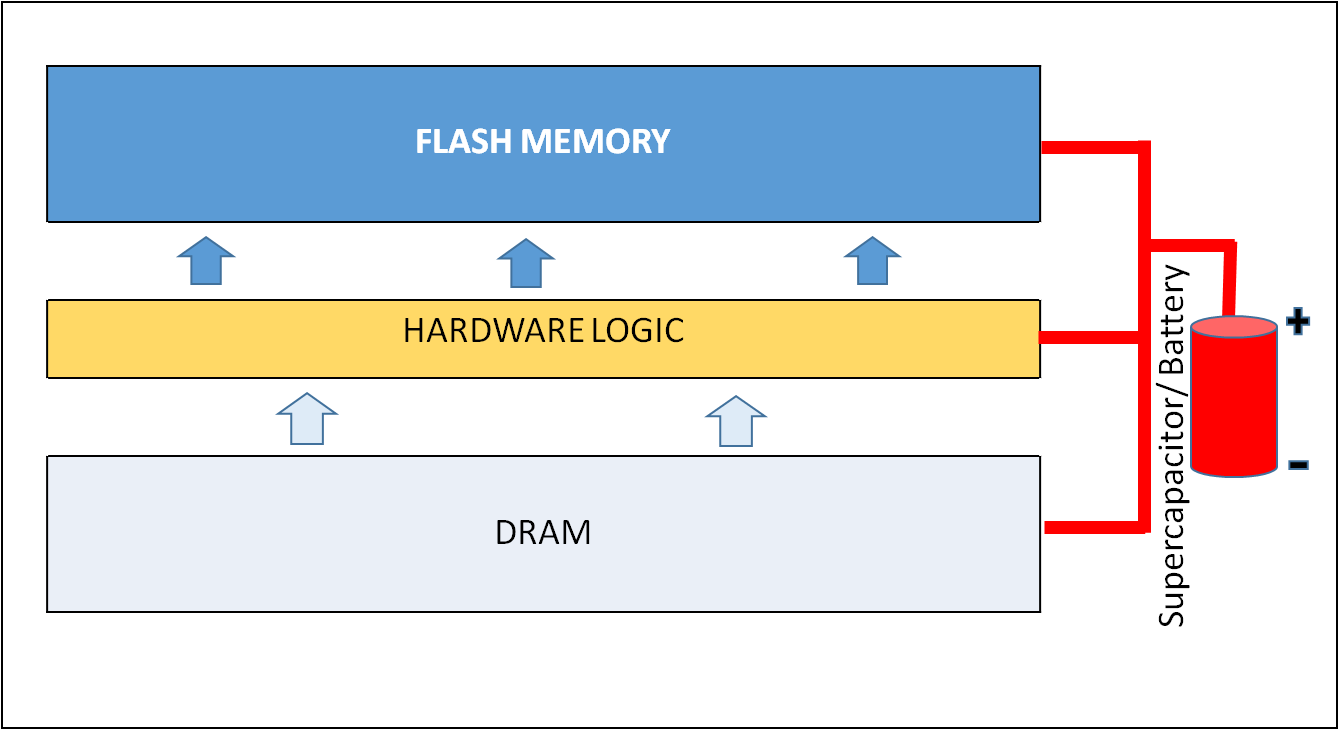
\includegraphics[scale=0.6]{figures/NVDIMM_Stack.png}
  \caption{NVDIMM Model}
  \label{fig:nvdimm}
\end{figure}
One of the key advantages is that NVDIMMs can function at DRAM speeds while providing non-volatility through background operations. Another important benefit is that both DRAM and flash are commercially mature technologies, combined simply by some hardware glue logic. 

\section{E820 Memory Map}

Devices external to the microprocessor can be broadly classified into two groups

1. I/O

2. Memory

The microprocessor interacts with these two devices in a similar way. I/O devices contain programmable registers, which act as an interface for the device, whereas memory is just a bank of byte addressable memory elements. Both memory and I/O read/write instructions are issued on the same bus, which are then forwarded appropriately by Northbridge chipset (See Fig~\ref{fig:intel_arch}). 

\setlength{\belowcaptionskip}{-10pt}

\begin{figure}[H]
  \centering
  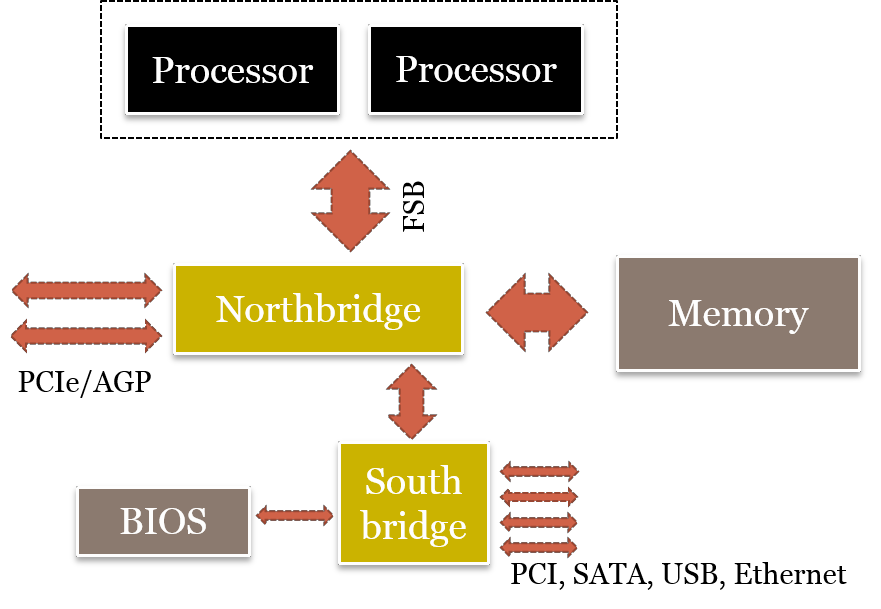
\includegraphics[scale=0.6]{figures/intelhubarchi.png}
  \caption{Intel Hub Architecture}
  \label{fig:intel_arch}
\end{figure}

In the nascent stages of microprocessor development different companies went with different I/O models. Intel included a separate I/O pin in its microprocessor which separated memory and I/O addresses into two separate address spaces, effectively providing an extra bit. For example if the ISA supported 16 bit addresses, we get one 16 bit address space for I/O and another 16 bit address for memory, which is the same as a 17 bit unified address space for both memory and I/O. Intel also had to provide a separate set of I/O instructions to manipulate I/O registers (called I/O ports) in its ISA. This address space segregation through an external I/O pin simplified the address decoding logic in Northbridge chipset. Moreover, then, addresses were just 16 bits wide, making the effective extra bit, a precious resource addition. On the downside, the ISA become more bulky with separate I/O instructions performing similar tasks as Memory instructions. 

On the other hand, Motorola provided a Memory Mapped I/O model. Here I/O registers and memory are mapped on to the same address space, each occupying distinct addresses.  

This eliminated the need for any separate I/O instructions to be included in the ISA. However, as a result the address decoding logic in the Northbridge chipset became more complex. Where, in the previous case the chipset just had to check the value of one bit (I/O pin of the microprocessor), here, it had to decode the entire address, to forward the instruction to the correct bus. Moreover this scheme had to share the address space between both memory and I/O. 

In the long run, many of the disadvantages of MMIO mentioned above disappeared, making it the dominant model used in today's computers. With scaling of transistor technology, hardware logic became inexpensive, and the Northbridge could easily handle the additional hardware for complete address decode logic. The address space also expanded from 16 bits to 32 bits and now on to 64 bits, which is more than enough for both memory and I/O. This model had a major advantage of preventing duplication of instructions at the ISA level. The vast plethora of memory management instructions are more comprehensive and can be used in the same way for I/O registers. Thus MMIO is more popular, with I/O ports, only supported for legacy reasons. 

This begs the question now, that how does the OS know the division of the address space between memory and I/O. The translation occurs at Northbridge, and differs from one motherboard to another. These hardware details are hidden in an abstraction layer provided by BIOS, in the form of E820 Memory Map. This list is generated by BIOS on raising a software interrupt 0x15, with EBX set to 0xE820. 

\setlength{\belowcaptionskip}{-10pt}

\begin{table}[H]
  \centering
  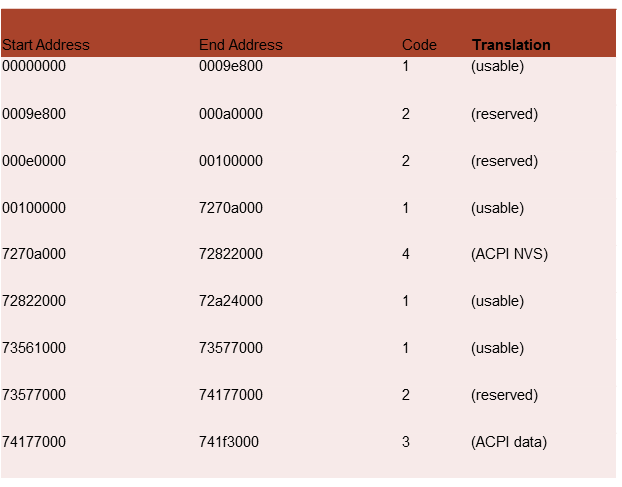
\includegraphics[scale=0.6]{figures/e820table.png}
  \caption{Sample E820 Table}
  \label{fig:e820table}
\end{table}

Physical address ranges are currently divided into 6 regions which are indicated by the type field.

A brief description of the different types is as follows:

1. AddressRangeMemory: Available RAM

2. AddressRangeReserved: Reserved by the system, generally contains I/O addresses.

3. AddressRangeACPI: Stores ACPI tables.

4. AddressRangeNVS: Not usable by the OS. This range is required to be saved and restored across an NVS sleep.

5. AddressRangeUnusuable: Memory regions containing errors.

6. AddressRangeDisabled: Memory not enabled.

7. Other :Undefined. Reserved for future use.

An E820 memory map contains a list of valid addresses. It serves the following basic services

1. Indicate the physical address space to the OS.

2. Indicating usable RAM regions.

3. Indicate I/O regions, corrupted memory regions, along with other reserved regions.

The first point is very important, since  on boot up the OS is unaware of the amount of memory and I/O devices present in the system. With the knowledge of the memory space the OS can then create page tables and other data structures, to use and share the memory. For the reserved I/O regions, there are several self-discovery mechanisms like Plug and Play (PnP) for devices to identify themselves along with their specific device addresses. 

\section{Intel VT extensions}
Popularity and demand for virtualization led Intel to introduce various features for the x86 platform, in VT-x and VT-d extensions. These extensions recognize the following additional modes of operation of the CPU. 

1. VMX root: This is the highest level of privilege only accessible to a VMM. 

2. VMX non-root: This mode is appropriate for guest VMs, containing all the typical privilege levels encountered by an OS in a non-virtualized environment. 

De-privileging an OS relies on extending the traditional framework between applications and OS, to OS and the hypervisor. Sensitive instructions which used to cause traps to the OS, would now trap to the VMX root. These transitions from VMX non-root mode to VMX root mode are termed as VM exits (the reverse is called VM entry). During a VM exit, the state of a guest machine (VM) is saved to, and the state of the host machine (VMM) is restored from, a Virtual Machine Control Structure (VMCS). VMCS is a hardware based memory structure (similar to page table structures) containing various regions defining the CPU state and behavior. It provides a hardware realization to the term vCPU, which was just an abstract concept earlier, realized entirely in software. Since the CPU state is saved to memory by hardware, it is much faster than prior software implementations of storing registers individually. VMCS structures also provide flexibility of masking VM exits on certain sensitive instructions. Interrupts may be remapped to a vCPU, eliminating the need for the VMM to first catch and then deliver these events to guests. 

Typically, applications indirectly gain access to system resources via system calls provided by the OS. These system calls were generally implemented using a software interrupt, which would change the privilege level of the CPU and transfer control of execution to a specific OS subroutine. To eliminate the overhead of a software interrupt and allow faster transitioning, Intel added a SYSENTER instruction which would result in a jump to a specified address in the MSRs. A similar functionality has been extended to hypervisors, especially to support paravirtualization. A special VMCALL instruction has been included in the VT-x extensions, which unconditionally causes a VM exit passing the control over to the VMM, in VMX non-root mode (/cite Intel reference manual). It differs from SYSENTER function in the sense that it stores the guest CPU state to the VMCS structure before moving to the hypervisor, while the SYSENTER instruction does not.  

VT-d instructions provide virtualization extensions for devices. It includes facilities such as IOMMU and interrupt remapping which when used in conjunction with VT-x reduce the overhead for I/O operations in virtualized environments. IOMMU has been easier to implement due to the incorporation of northbridge chipset inside the CPU itself. Earlier, memory controllers used to reside on the northbridge chipset external to the CPU. However, due to MOS scaling effects, memory controllers have been moved to the CPU die, and it is a lot easier to support a memory management unit for device memory accesses. VT-d extensions also provide for interrupt remapping capabilities to vCPUs, rather than physical CPUs further minimizing hypervisor intervention. 

These extensions are still an ongoing development, with each revision providing newer features and trying to close the gap between virtualized and non-virtualized environments. Hypervisors are also continually evolving to making extensive use of the added capabilities.

%%%INCLUDE FIGURES OF COMPUTER MODEL WITH NORTHBRIDGE

%\include{combined}

%\section{Related Work}

Many works have attacked this problem using different design techniques.
In Kandoo{[}{]}, the authors propose a hierarchical controller design,
where the local applications are offloaded to the local controllers,
while the applications requiring global view of the network, execute
on a centralised one. The design requires maintenance of complex data
structures between the global and local controllers. The Difane{[}{]},
presents a TCAM expensive solution, where the secondary switches acts
as cache devices. It partitions the flows among a set of switches
and installs appropriate rules, to selectively direct packets to specific
switches. NOSIX aids the applications running on the controller with
a view of the virtual flow tables. However, it relies on the vendor
to provide an interface of updating virtual to physical tables. The
work on {[}{]}(Rexford Paper) tries to solve the \textquotedblleft{}infinite
flow\textquotedblright{} capacity problem, by extending its work on
the Difane paper. It exploits the large data capacity of software
switches by using them as the secondary cache devices. It requires
the complex overhead of creating it\textquoteright{}s own rules which
forms the basis of selectively directing packets to the specific software
switches on a hardware switch miss.

In our SDN architecture, the flowcache acts a proxy device which avoids 
the complexity of creating new rules by installing rules which are inserted 
by the controller. In this paper, we present a novel architecture, in line 
with the memory system architecture to achieve the required performance goals.


\chapter{\uppercase{Xen Hypervisor}}
Xen is an open-source hypervisor, that started as a project at University of Cambridge. It uses paravirtualization in conjunction with hardware assisted virtualization technologies to develop a VMM. Along with widespread adoption, it also boasts of native support from Linux kernel. 

\section{Xen Architecture}

Xen hypervisor follows a minimalist design policy with emphasis on security and efficiency. This is extremely important as the hypervisor hosts multiple Virtual Machines and any bugs may compromise the entire system. Virtual machines are hosted on custom environments called domains. Xen exposes very basic functionalities to these domains having similar UNIX counterparts as shown in Table~\ref{tab:unixcomp}. Guest OSes should contain relevant modifications to use these features. 

\begin{table}[H]
\centering
%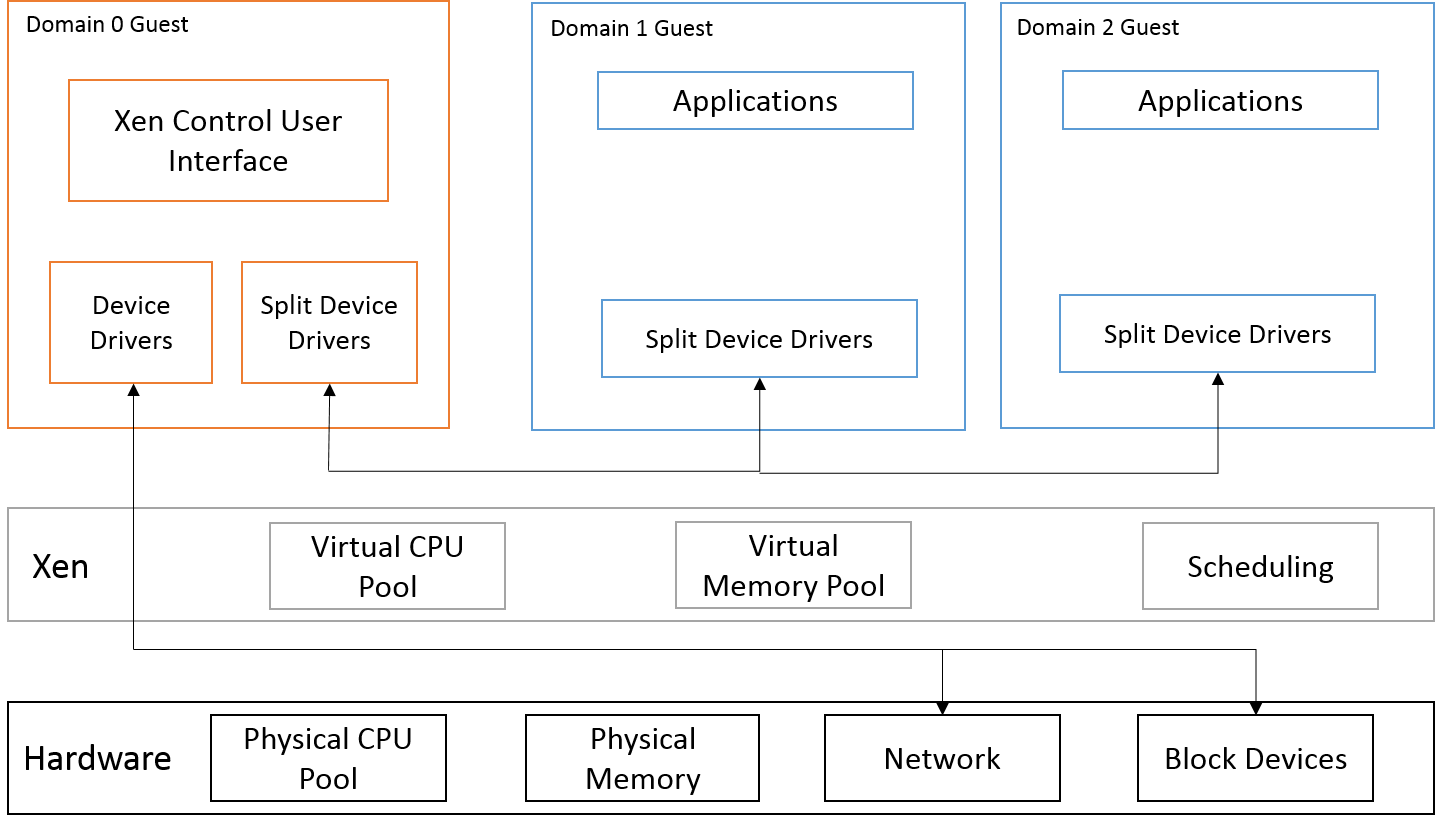
\includegraphics[scale=0.6]{figures/Xen_model.png}
\begin{tabular}{|c|c|}
    \hline
    UNIX & Xen \\
    \hline
    \hline
    System Calls & Hypercalls \\
    \hline
    Signals & Events \\
    \hline
    File system & Xenstore \\
    \hline
    POSIX shared memory & Grant tables  \\
    \hline
\end{tabular}
\caption[Comparison between Xen and Unix architecture]{Comparison between Xen and Unix architecture \cite{chisnall_book}}
\label{tab:unixcomp}
\end{table}

Initially Xen was designed undertaking paravirtualization on x86, i.e. Guest OS kernels were modified to be compatible with Xen. However, with the addition of Intel VT-x and AMD SVM extensions to the x86 architecture, it is possible to support pure virtualization. Guests on newer machines can run in two modes -- PV (Paravirtual) guest or HVM (Hardware Virtual Machine) Guest. In HVM mode, Xen can run guests without any source code modifications. On the other hand, running a paravirtualized guest kernel in HVM takes the hybrid approach where the guest may take advantage of hardware features (such as Nested Page Tables), in addition to the performance boosts provided by paravirtualization techniques (such as hypercalls). Guests can use the CPUID instruction to probe whether it is running directly on hardware, or on top of Xen.

The trap and emulate model, for hypervisors, is very expensive in terms of CPU cycles. Thus sensitive operations in a guest OS are typically replaced with hypercalls. This is quite similar to system calls in UNIX. Typically system calls use interrupt 80h (or SYSENTER instruction) to transfer control to the kernel in ring 0 with arguments either placed on the stack or in ISA registers. Hypercalls work in much the same way utilizing interrupt 82h instead in PV mode. However, in HVM mode, most interrupts are generally configured to be fed to the guest kernel instead of Xen. To enter the hypervisor at ring -1, a special instruction, VMCALL, is used instead.

These two separate methods are unified in newer Xen versions via calling an address at a certain offset in a special page mapped to the Guest OS's address space. The offset determines the specific hypercall command. In the above method, the hypercall issue procedure remains the same from the Guest OS kernel's perspective whether in PV mode or in HVM mode. The implementation specifics are hidden in the page mapped to the Guest VM.

In a Xen based system (Fig \ref{fig:xen_model}), memory and CPU resources are managed directly by the hypervisor, but I/O devices are generally controlled using a privileged domain (generally dom0). This domain runs at a higher privilege level where it is given direct access to many hardware resources. In addition to handling I/O operations, it also hosts the Xen User Interface used for administrative tasks. Thus, its security is of prime importance. Some of its responsibilities, such as hosting a device driver, may be delegated to domU guests (Guest domains) running at a higher privilege level. This feature is very useful in the case of a buggy device driver, as during any device driver related fault, only the specific domU needs to be restarted instead of the entire system. However, in the absence of IOMMU, DMA requests from this domain may potentially affect memory regions allocated to other VMs. 

\begin{figure}[H]
\centering
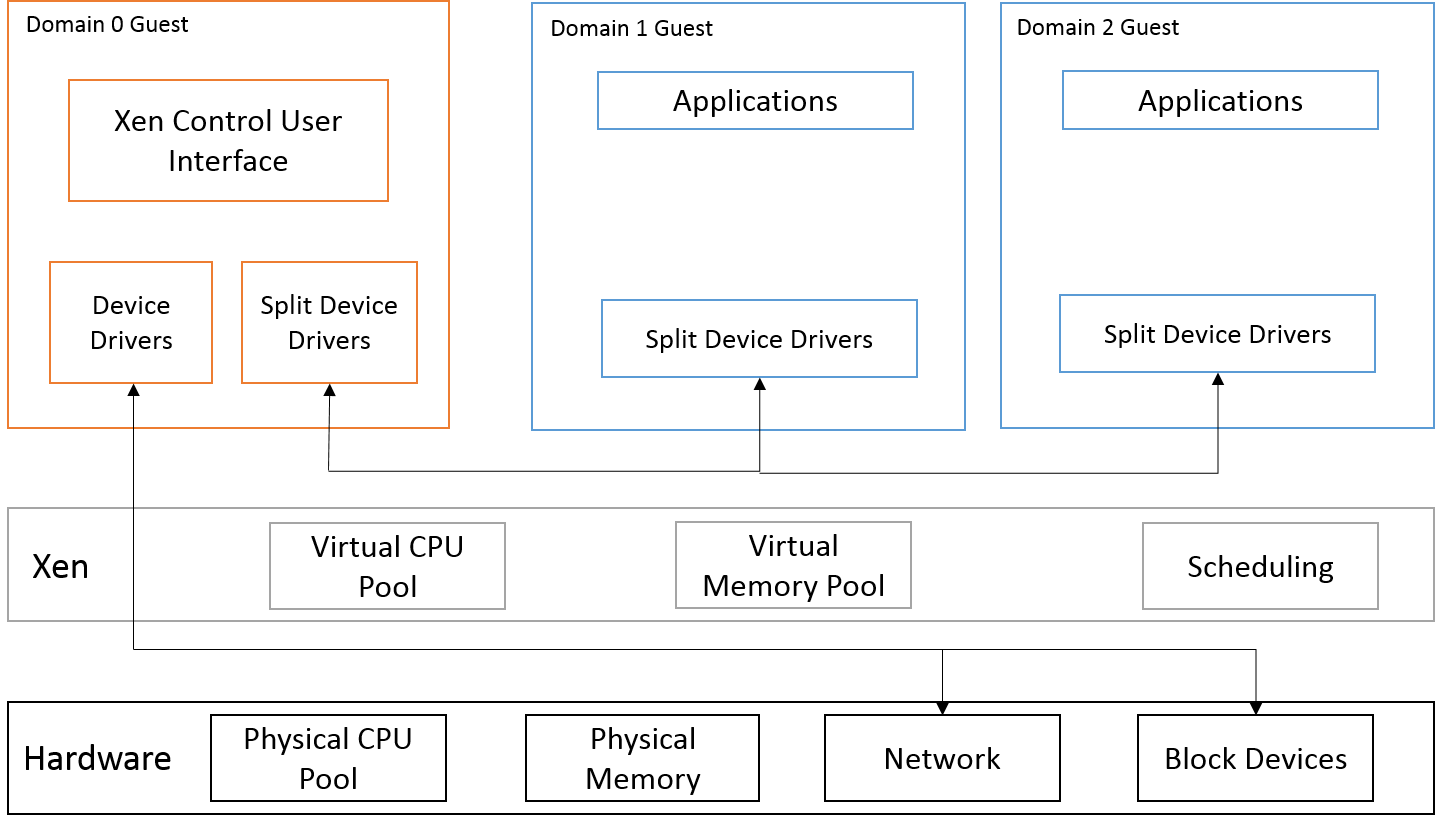
\includegraphics[scale=0.6]{figures/Xen_model.png}
\caption[Xen Architecture]{Xen Architecture \cite{chisnall_book}}
\label{fig:xen_model}
\end{figure}
Memory sharing in Xen is enabled via Grant tables. Memory is shared or transferred among domains at page granularity. This feature is quite useful in many situations such as networking among guests and implementing split device driver model.

One of the features of Xen which makes it very popular is its I/O interface. Xen escapes the need to both emulate devices and develop separate device drivers with a split device driver model. It is made up of the following.

1. Actual device driver.

2. Generic backend driver.

3. Generic frontend driver.

4. Ring buffer.

Typically, dom0 or a driver domain hosts the actual device drivers eliminating a notable amount of redundant developmental work. A generic frontend device driver is implemented in the guest domain at a much higher abstraction level which communicates with the backend device driver using ring buffers. The backend driver deconstructs the I/O requests from the front end driver and forwards it to the actual device driver. The requests are thus kept very simple avoiding device specific details. Ring buffers handle data movement across domains using shared memory utilities provided by Xen (Grant tables). A key advantage of this model is that a single split device driver can cover a whole class of devices.

Time keeping is another important aspect of an Operating System, especially for a scheduler. CPUs are shared amongst the running processes on a time sharing basis, and thus it is of utmost importance that the Operating System has accurate CPU clock information. Additionally, several user space applications also need wall clock time information, which can be calculated from system time. Usually the above is gathered using the CPU clock and network time information. However, in a virtual machine the CPU clock does not reflect the system time, because different Operating Systems share the same CPU. The hypervisor holds the responsibility to provide a virtual machine with system time corresponding to the actual time the VM occupies a CPU. In HVM domains, Xen receives support from the hardware extensions, while in PV domain the above is performed entirely in software. 

\section{Xen Control Interface}
The control interface of Xen contains a combination of user space, and kernel space code, through which hypercalls are issued. To host the interface, dom0 must comprise of a compliant kernel (Linux, NetBSD, Solaris, etc.) containing requisite modifications. The process stack, including and above the Xend daemon (Fig \ref{fig:xen_api}), run as user space applications while the rest run at a higher privilege level. 

\begin{figure}[H]
\centering
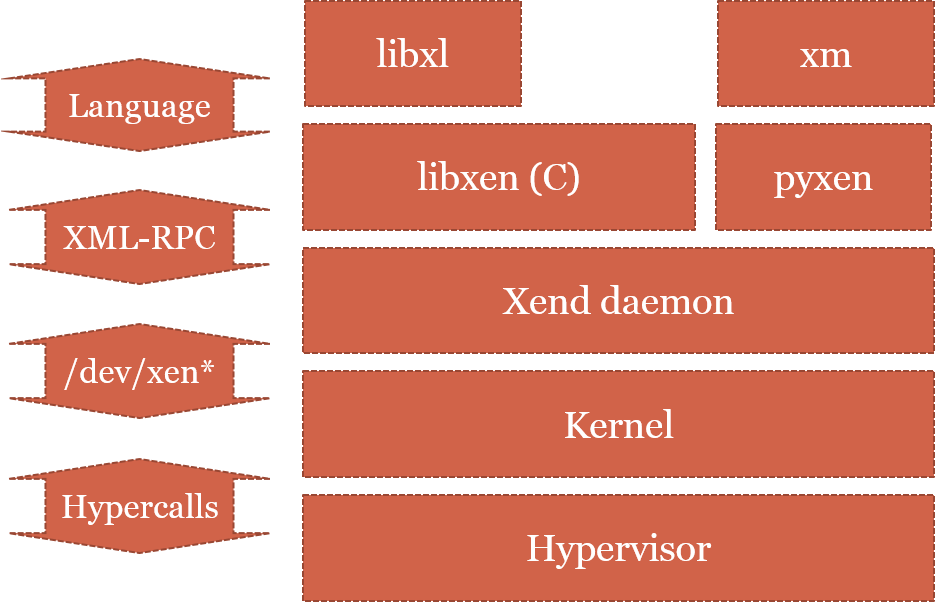
\includegraphics[scale=0.7]{figures/XEN_API.png}
\caption[Xen API]{Xen API \cite{chisnall_book}}
\label{fig:xen_api}
\end{figure}
Xen commands issued through any tool, are converted to XML-RPC messages to communicate with the Xend daemon. Xend daemon forwards the command to the kernel to issue hypercalls. In this chain of flow, the interface of Xend daemon is standardized through the definition of Xen API. This allows development and proliferation of user space management tools independent of changes lower in the stack. The complete Xen Control Interface structure is presented in Fig \ref{fig:xen_api}. Xen commands can be issued from a variety of user space tools such as xl, xm, libvirt, etc. Some tools (e.g. xm) written in python, have an additional overhead of a runtime python environment. In contrast, xl is relatively lightweight using libxen library, written in C, to generate XML-RPC messages.

The xend daemon runs in the user space, thus minimizing dependence on a specific kernel. On receiving messages, xend performs certain critical tasks such as access control and issues hypercalls to the hypervisor through the kernel.

Sample commands for xl toolchain are illustrated below:

\begin{itemize}
\item Create or start a virtual machine: xl create \textless config\_filename\textgreater

\item Shutdown a virtual machine: xl shutdown \textless domain\_id\textgreater
\end{itemize}


\section{Xen Memory Model}

Memory management is one of the core components of a hypervisor. With Xen core, the available memory is shared dynamically amongst the different virtual machines. It also allows for thin provisioning, i.e., projecting more memory than the available system RAM using ballooning techniques.

As a part of design philosophy, Xen does not swap pages out of memory itself. Individual guest OSes’ are the best judges to identify cold pages and thus this job is left over to them. Using the balloon driver, Xen is able to mount or release memory pressure in a VM. When the hypervisor wants to reclaim pages from a VM, it inflates the balloon driver in the virtual machine. The balloon driver requests more memory from the OS, which swaps cold pages out and releases memory to the balloon driver. The latter returns those freed up memory pages to the hypervisor so that it can be allocated to an appropriate VM. During runtime, as the memory requirement reduces, Xen deflates the balloon and releases memory back to the VM. The balloon driver monitors a target memory value, set in Xenstore to dynamically balance the actual memory allocated to the guest. This target memory value (set through domain0) is usually smaller than the guest physical address space and reflects the intended actual memory allocation for that domain. 
 

\subsection{x86\_64 Memory management}
This subsection focuses on the memory management details for x86\_64 machines. While extending the x86 ISA to 64 bits, AMD cleaned up memory segmentation controls, leaving a continuous flat address space with page level controls. In x86\_64, virtual memory is 64 bits wide, currently allowing only 48 bit sign extended addresses \cite{intel_manual}. A typical system looks similar to Fig \ref{fig:x86_memspace}, having 128TB + 128TB accessible regions. 

\begin{figure}[H]
\centering
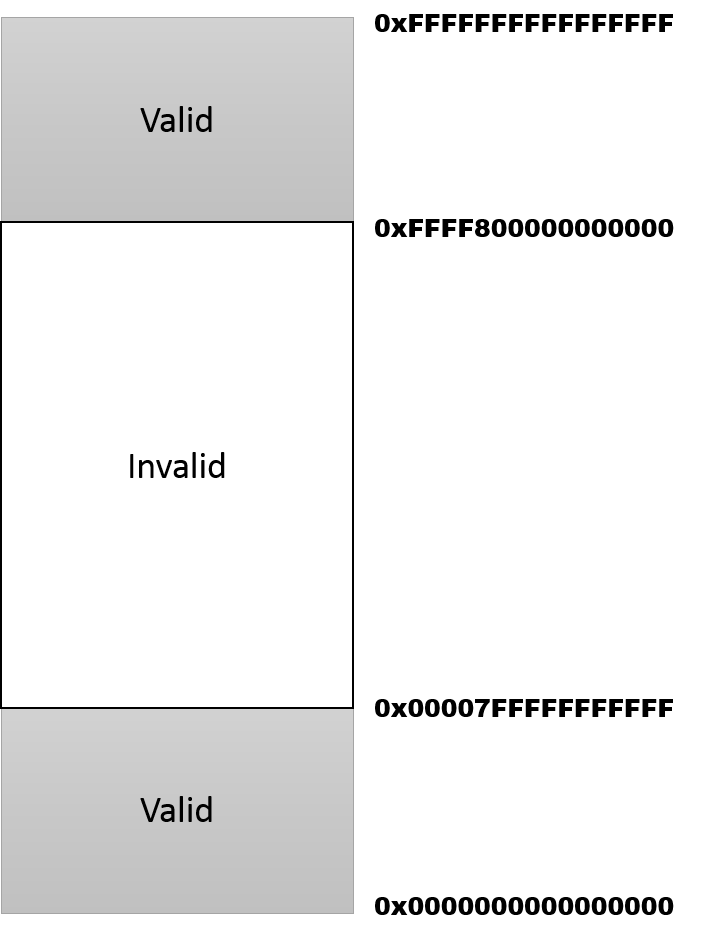
\includegraphics[scale=0.6]{figures/x86_64_VA_space.png}
\caption{x86\_64 Virtual Address Space}
\label{fig:x86_memspace}
\end{figure}

Typically for most Operating Systems, a virtual address space is generally divided into two parts

1. Kernel Space: This space is shared and common to all the applications. Kernel space also contains a direct mapping of the physical address space (usually with an offset).

2. Application Space: This space is specific to individual applications for application data and code.

For Linux on x86\_64 machines, the lower region goes to the application and the upper region is occupied by the kernel. Mapping the kernel into the individual application address spaces avoids the overhead of a context switch during a system call. Moreover, many system calls pass arguments via a pointer to a user space memory region, that is also accessible directly by the kernel, since the kernel is mapped onto the process address space. 

\begin{figure}[H]
\centering
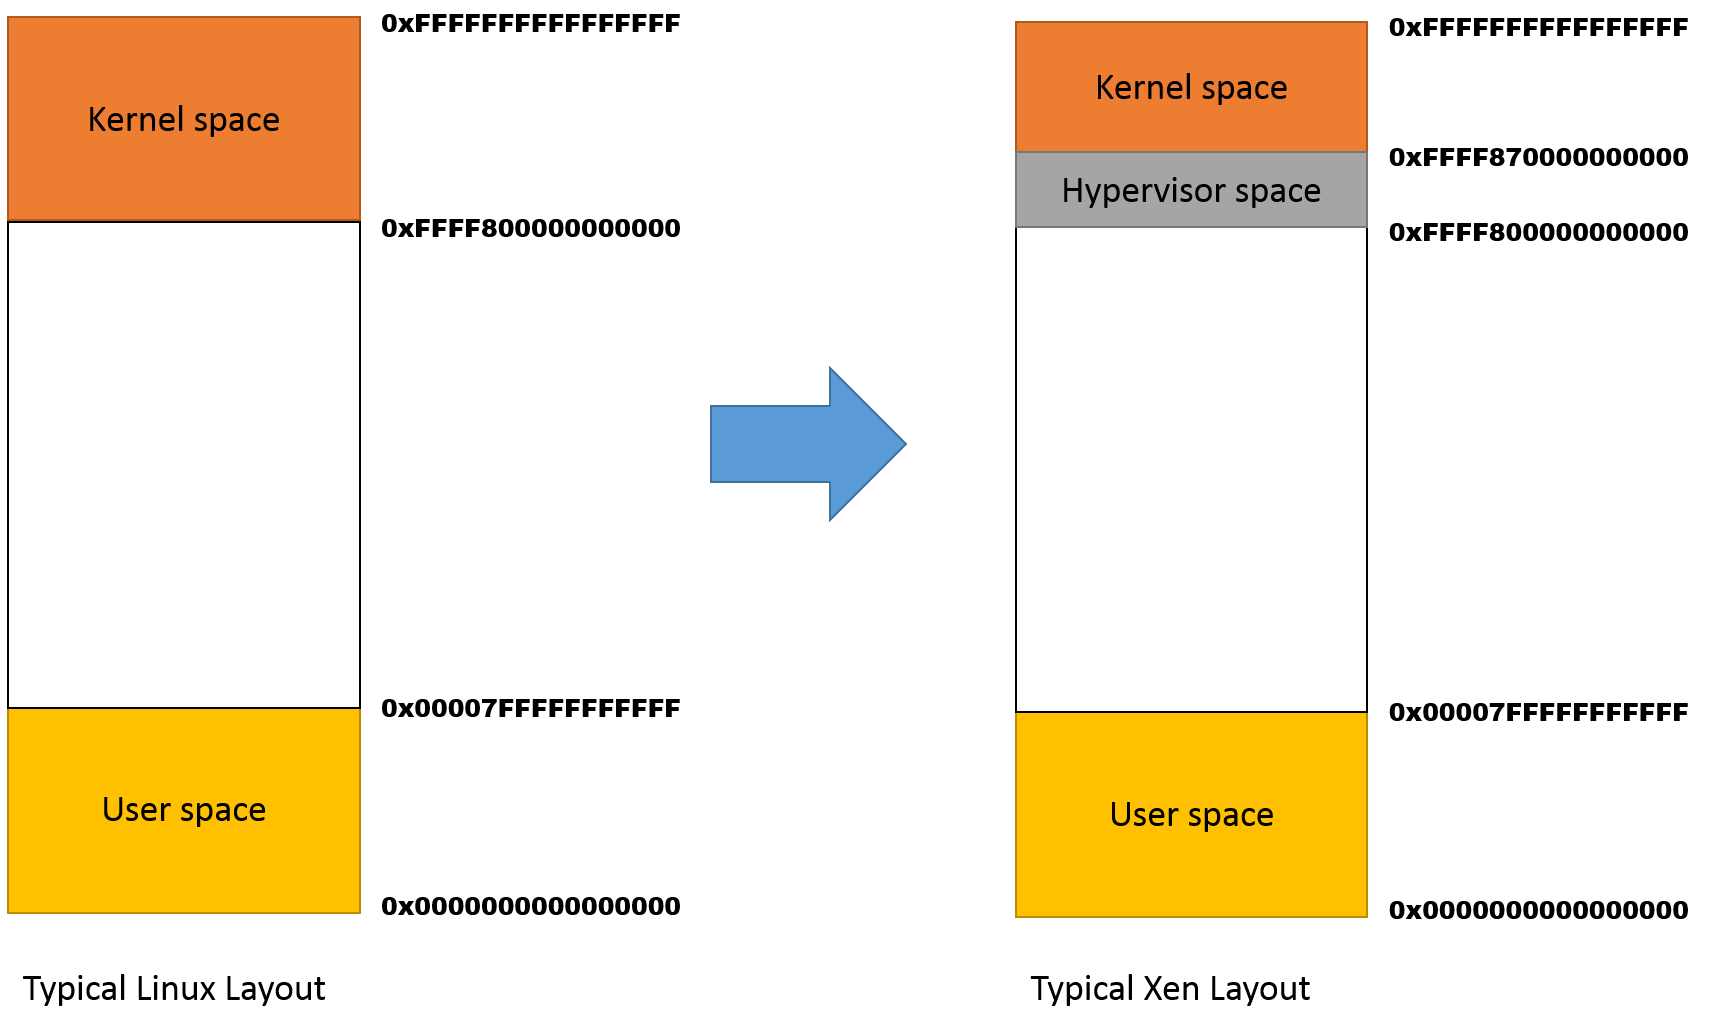
\includegraphics[scale=0.7]{figures/VA_layout_hypervisor.png}
\caption{Xen Virtual Address Layout Transformation}
\label{fig:xen_layout}
\end{figure}

A similar framework is setup in-between Xen hypervisor and the individual VMs (see Fig \ref{fig:xen_layout}). The hypervisor reserves a portion of the kernel address space for itself. This is done again to avoid context switches during hypercalls from a guest VM. This address space is again subdivided into different regions. 

%\begin{table}
%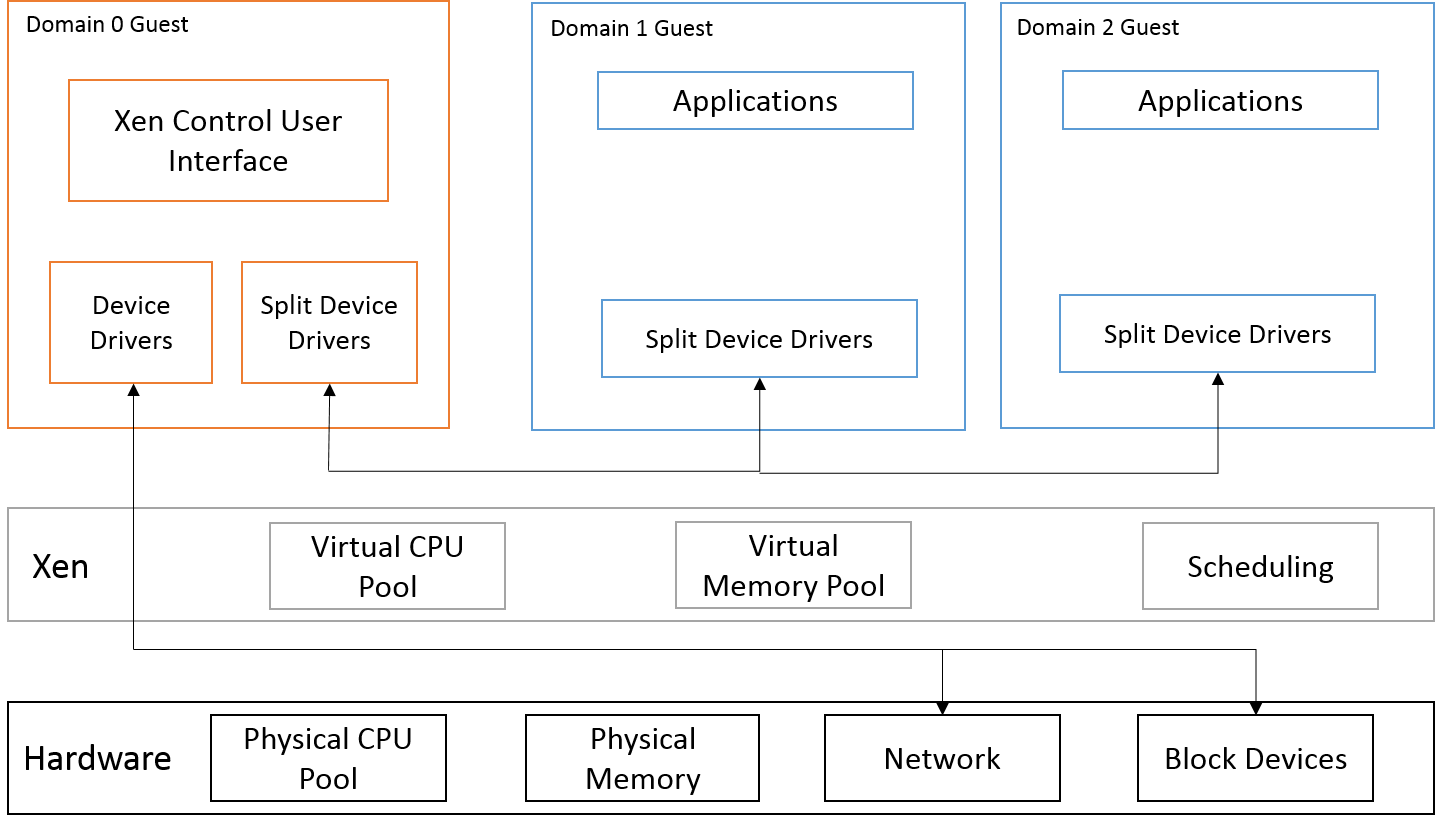
\includegraphics[scale=0.6]{figures/Xen_model.png}
\clearpage
\begin{longtable}{|m{2ex}|m{20ex}|m{18ex}|m{0.39\textwidth}|}
    \caption[Virtual Memory Regions]{Virtual Memory Regions \cite{xen_code} \label{tab:xen_address}}\\
    \hline
    & Start Address      & End Address        & Description \\
    \hline
    \hline
    \endfirsthead
    \hline
    \multicolumn{4}{|c|}{Continuation of Table \ref{tab:xen_address}}\\
    \hline
    \hline
    & Start Address      & End Address        & Description \\
    \hline
    \hline
    \endhead
    \hline
    \hline
    \multicolumn{4}{|c|}{\textit{Continued...}}\\
    \hline
    \endfoot
    \hline
    \hline
    \multicolumn{4}{|c|}{End of Table \ref{tab:xen_address}}\\
    \hline
    \endlastfoot
    1  & 0x0000000000000000  & 0x00007fffffffffff & [128TB, PML4:0-255] Guest-defined use \\
    \hline
    2  & 0x0000800000000000  & 0xffff7fffffffffff & [16EB] Inaccessible: Only 48-bit sign-extended VAs supported\\
    \hline
    3  & 0xffff800000000000  & 0xffff800000000000 & [256GB, PML4:256] Read-only machine-to-phys translation table (GUEST ACCESSIBLE) \\
    \hline
    4  & 0xffff804000000000  & 0xffff807fffffffff & [256GB, PML4:256] Reserved for future shared info with the guest OS (GUEST ACCESSIBLE) \\
    \hline
    5  & 0xffff808000000000  & 0xffff80ffffffffff & [512GB, PML4:257] ioremap for PCI mmconfig space \\
    \hline
    6  & 0xffff810000000000  & 0xffff817fffffffff & [512GB, PML4:258] Guest linear page table \\
    \hline
    7  & 0xffff818000000000  & 0xffff81ffffffffff & [512GB, PML4:259] Shadow linear page table \\
    \hline
    8  & 0xffff820000000000  & 0xffff827fffffffff & [512GB, PML4:260] Per-domain mappings (e.g., GDT, LDT) \\
    \hline
    9  & 0xffff828000000000  & 0xffff82bfffffffff & [256GB, PML4:261] Machine-to-phys translation table \\
    \hline
    10 & 0xffff82c000000000  & 0xffff82c3ffffffff & [16GB, PML4:261] ioremap()/fixmap area \\
    \hline
    11 & 0xffff82c400000000  & 0xffff82c43fffffff & [1GB, PML4:261] Compatibility machine-to-phys translation table \\
    \hline
    12 & 0xffff82c440000000  & 0xffff82c47fffffff & [1GB, PML4:261] High read-only compatibility machine-to-phys translation table \\
    \hline
    13 & 0xffff82c480000000  & 0xffff82c4bfffffff & [1GB, PML4:261] Xen text, static data, bss \\
    \hline
    14 & 0xffff82c4c0000000  & 0xffff82f5ffffffff & [197GB, PML4:261] Reserved for future use \\
    \hline
    15 & 0xffff82f600000000  & 0xffff82ffffffffff & [40GB, PML4:261] Page-frame information array \\
    \hline
    16 & 0xffff830000000000  & 0xffff87ffffffffff & [5TB, PML4:262-271] 1:1 direct mapping of all physical memory\\
    \hline
    17 & 0xffff880000000000  & 0xffffffffffffffff & [120TB, PML4:272-511] Guest-defined use.  \\
\end{longtable}

As seen in Table \ref{tab:xen_address}, different regions, serve individual purposes, while the complete machine memory is made directly accessible to Xen through region 16. 

\subsection{Hypercalls}

Several hypercalls are provided to facilitate common memory management operations in Xen. Although in a pure virtualization environment, it is not necessary, but hypercalls are included for performance gains.

Page table management is one of the most expensive operations in a paravirtualization approach. To prevent direct access to physical hardware, page tables of a domain are generally marked as read only by the hypervisor. Any attempted modifications by the guest VM would result in a trap to the VMM, which then emulates the required operation.

Xen provides hypercalls for the guest to make the above procedure easier. It also allows for multiple page table changes to be clubbed together, via the HYPERVISOR\_mmu\_update hypercall. However, these operations are not relevant to the case of an HVM guest. In x86 architecture, the VT-x (for Intel chips) and SVM (for AMD chips) extensions allow the guest direct access to its own page tables. This eliminates the scenario for traps altogether.

Thin provisioning is another important feature in a virtual machine. The balloon driver negotiates the actual memory occupied by a domain with the hypervisor. The popular commands used by it are XENMEM\_increase\_reservation, XENMEM\_decrease\_reservation and XENMEM\_populate\_physmap. The first two are used for runtime addition or removal of memory blocks behind the guest physical address space. While the third one is used for the initial mapping of the guest address space during domain creation, for large memory requests. These commands are executed through the HYPERVISOR\_memory\_op hypercall. Another important command associated with this hypercall is XENMEM\_memory\_map. It can replace the BIOS call to provide an E820 memory map to a paravirtualized guest. Though not necessary for domU guests, it is one of the available ways to determine the initial layout of guest physical address space. 


\chapter{\uppercase{Design and Implementation}}

Conception of the proposed system revolves around the design of an additional memory management unit in the hypervisor. Since NVM data has existence beyond the lifetime of a VM, the conventional MMU cannot be used. A new Non-volatile memory management unit is presented as a solution, for a popular hypervisor -- Xen.

In this chapter, several features of Xen are described relevant to the x86\_64 ISA with VT-x extensions and Intel Hub Architecture, followed by requisite modifications to incorporate the new MMU design. 

\section{Overview}
Boot procedure on x86 demands that the CPU should first transition from real mode to protected mode to access the entire address space. It should initialize the necessary page table data structure and segment registers to perform the switch while keeping interrupts masked during the transition process. After entering the protected mode the processor has a lot more flexibility, but typically loses access to BIOS calls. For the above mentioned reasons, bootstrapping on x86 is a quite complex and tricky procedure. Typically, initialization of a MMU is one of the first tasks for any kernel, and it involves a fair amount of bootstrapping code. It makes this undertaking all the more challenging and interesting.

Booting can also designate either the host machine startup or just starting a virtual machine. While the former is associated with the hypervisor taking stock of the hardware resources, the latter involves sharing the same with a VM in a secure manner. The major steps performed in a Xen based system from power on to starting a new domain is summarized in the flowchart presented in Fig \ref{fig:xen_flowchart} and Fig \ref{fig:dom_flowchart}. As evident from this figure this project can be broken down into two fundamental subdivisions.

1. Create an independent Memory Management Unit for the available Non-Volatile RAM.

2. Provide guest domains access to the NVRAM region, in a secure and protected manner. 


\begin{figure}[H]
\centering
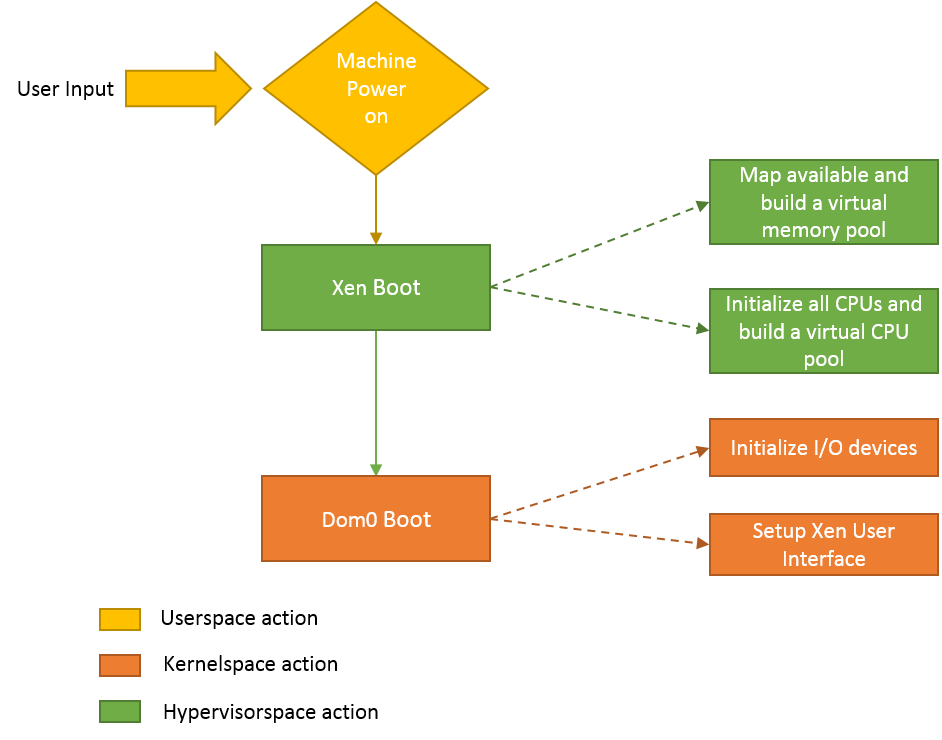
\includegraphics[scale=0.9]{figures/domain_creation1.png}
\caption{Domain Creation Flowchart : System Boot}
\label{fig:xen_flowchart}
\end{figure}

\begin{figure}[H]
\centering
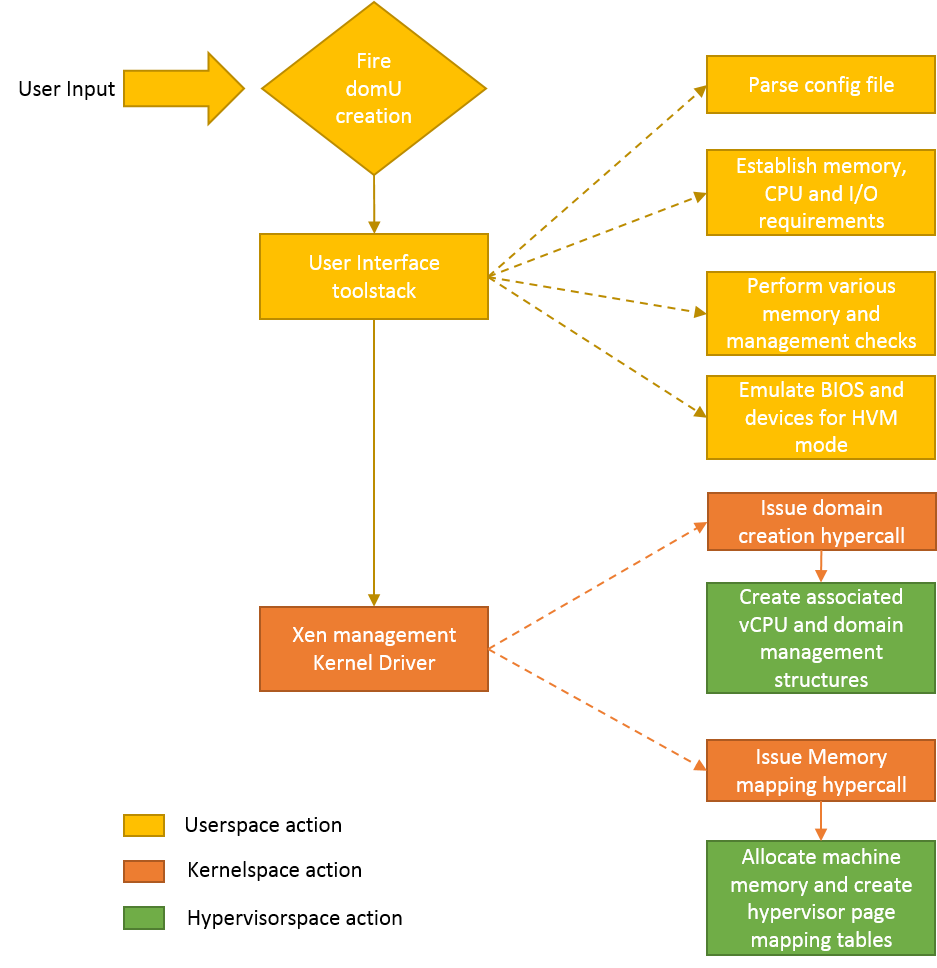
\includegraphics[scale=0.9]{figures/domain_creation2.png}
\caption{Domain Creation Flowchart : DomU Boot}
\label{fig:dom_flowchart}
\end{figure}
The first task requires modifications in the Xen kernel, with parts that deal with the boot process. Since the modifications are at the highest privilege level, it is very critical that the implementation be bug free, secure and efficient. Even minor bugs may cause the entire system to crash.

On the other hand, the second job deals more with user level code, specific to a toolchain. A notable part of domain creation focuses on emulation of firmware, performed mainly by various management tools. Only a small portion deals with issuing hypercalls for resource allocation. Therefore, in this section most of the implementation details reside in the Xen control interface with minor modifications to the hypercall structure. Due to standardization of Xen API, many tools have sprung up for VM management. This implementation picks up the xl toolchain, which is the default tool supported by Xen community.

A basic outline of the implementation is presented below, in Fig \ref{fig:xen_mod}, highlighting the modifications in red.

1. Recognize the presence of NVRAM from E820 memory map provided by BIOS.

2. Create a separate NVRAM pool to manage the resource independently.

3. Create separate interface to specify DomU RAM and NVRAM requirements.

4. Generate virtual E820 memory map reflecting the separate NVRAM pool.

5. Map the virtual NVRAM space in domUs to the physical Non-volatile memory present on the machine. 

\begin{figure}[H]
\centering
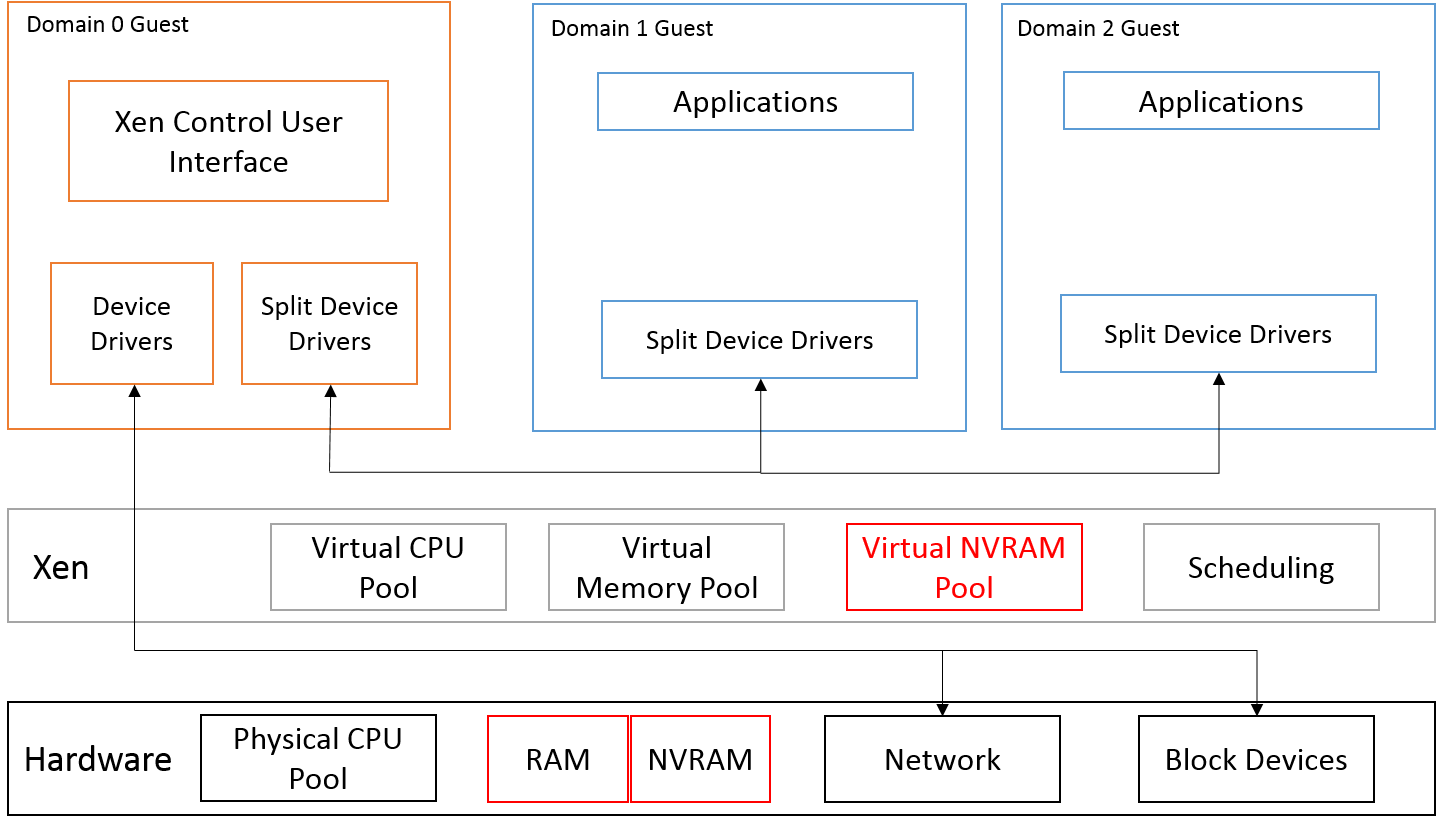
\includegraphics[scale=0.6]{figures/Xen_mod_model.png}
\caption{Modified Xen Architecture}
\label{fig:xen_mod}
\end{figure}

\section{Challenges}

There are several challenges faced during the design of the proposed system in Xen. The most notable being the absence of a modular design for system memory. Xen has been architected around volatile memory, and the notion of a homogeneous memory is integrated quite deep in the system design. This makes it all the more challenging to introduce another MMU. Moreover, a major portion of the initialization is done during the boot procedure, which is in itself quite a complex process for x86. Along with the above virtualization being a relatively new technology lacks sufficient documentation. Thus, even minor code changes turn into a grueling task. The combination of the above issues makes the implementation an arduous but exciting challenge. 


\section{Xen Boot Procedure}
On system start, Xen boots up first to take stock of the hardware present. It queries the BIOS for the E820 Memory map. Identifying the available memory regions, Xen builds preliminary page tables and switches the machine to protected mode. With paging enabled, the hypervisor can access the entire address space. It follows by building free page lists.

Each machine page is identified by a data structure called page\_info presented below \cite{xen_code}. This structure contains runtime administrative information about the machine pages such as status, domain identifier, special page status, order, etc. An array of these structures is initialized for all the machine pages as indicated in Fig \ref{fig:page_info_mapping}. This array of struct page\_info occupies the region 15 of Xen virtual address space identified in Table \ref{tab:xen_address}. Xen modifies this data structure to indicate any changes to the machine page. With predefined virtual address space regions for both the page\_info structures and the machine pages, a pointer to this structure can be used to calculate the virtual address of the corresponding page and vice versa. 

\smallskip
\begin{lstlisting}

 struct page_info
 {
     union {
         struct page_list_entry list;
         paddr_t up;
         uint64_t shr_handle;
     };
     /* Reference count and various PGC_xxx flags and fields. */
     unsigned long count_info;
     /* Context-dependent fields follow... */
     union {
         /* Page is in use: ((count_info & PGC_count_mask) != 0). */
         struct {
             /* Type reference count and various PGT_xxx flags and fields. */
             unsigned long type_info;
         } inuse;
         /* Page is in use as a shadow: count_info == 0. */
         struct {
             unsigned long type:5; /* What kind of shadow is this? */
             unsigned long pinned:1; /* Is the shadow pinned? */
             unsigned long head:1; /* Is this the first page of the shadow? */
             unsigned long count:25; /* Reference count */
         } sh;
         /* Page is on a free list: ((count_info & PGC_count_mask) == 0). */
         struct {
             /* Do TLBs need flushing for safety before next page use? */
             bool_t need_tlbflush;
         } free;
     } u;
     union {
         /* Page is in use, but not as a shadow. */
         struct {
             /* Owner of this page (zero if page is anonymous). */
             __pdx_t _domain;
         } inuse;
         /* Page is in use as a shadow. */
         struct {
             /* GMFN of guest page we're a shadow of. */
             __pdx_t back;
         } sh;
         /* Page is on a free list. */
         struct {
             /* Order-size of the free chunk this page is the head of. */
             unsigned int order;
         } free;
     } v;

     union {
         u32 tlbflush_timestamp;
         struct {
             u16 nr_validated_ptes;
             s8 partial_pte;
         };
         u32 shadow_flags;
         __pdx_t next_shadow;
     };
 }; 


\end{lstlisting}
 
\begin{figure}[H]
\centering
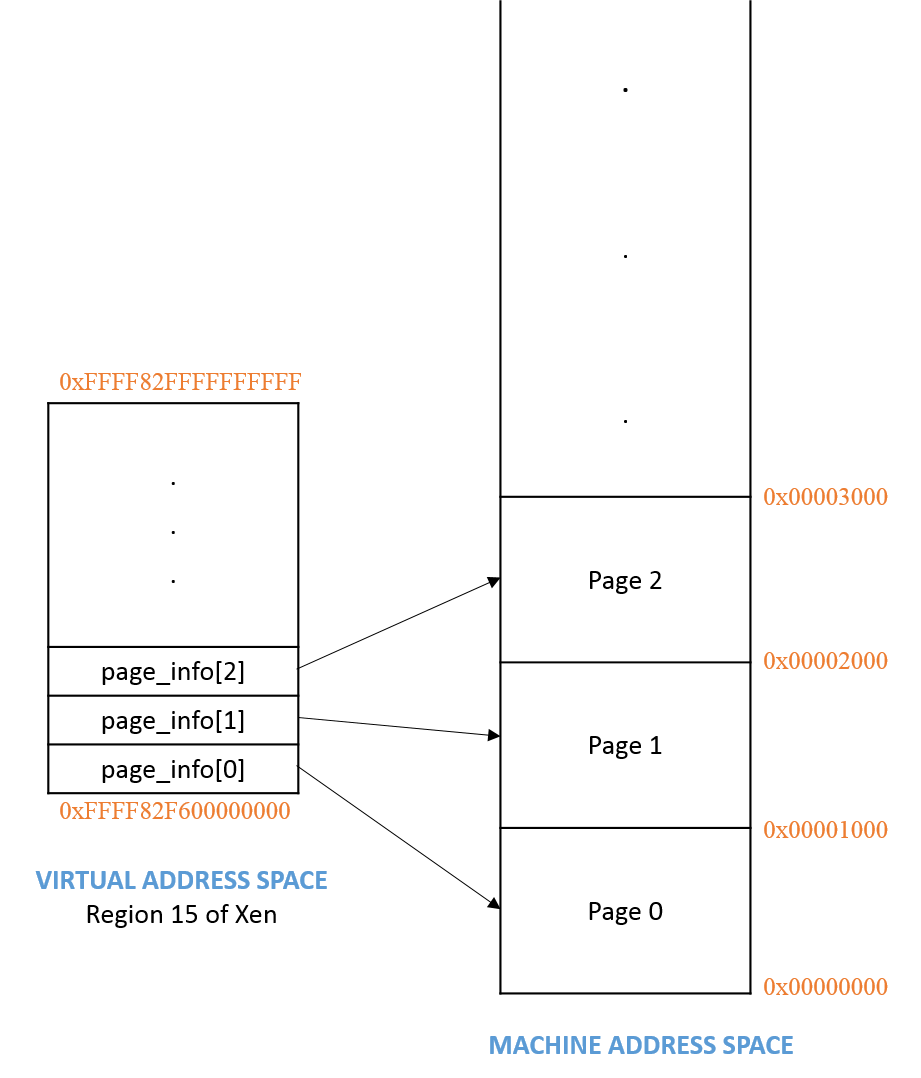
\includegraphics[scale=0.8]{figures/page_info.png}
\caption[Struct page\_info array to Machine Page mapping]{Struct page\_info array to Machine Page mapping \cite{xen_code}}
\label{fig:page_info_mapping}
\end{figure}

On system boot up, all the machine pages are free, without any domain affiliations. The Memory Management Unit builds a memory pool data structure \_heap[MEMZONE][ORDER] to manage and assimilate all the free pages. This \_heap data structure (Fig \ref{fig:heap_struct}) represents the free memory pool in Xen, arranging all the pages by MEMZONE and ORDER. Here MEMZONE divides the entire machine address space into different zones based on the position of the first non-zero bit in the address. This is necessary for special DMA memory requests for devices with fewer address bits. In each ZONE the pages are sorted by the order of the contiguous available pages up to a maximum of 1GB. 


\begin{figure}[H]
\centering
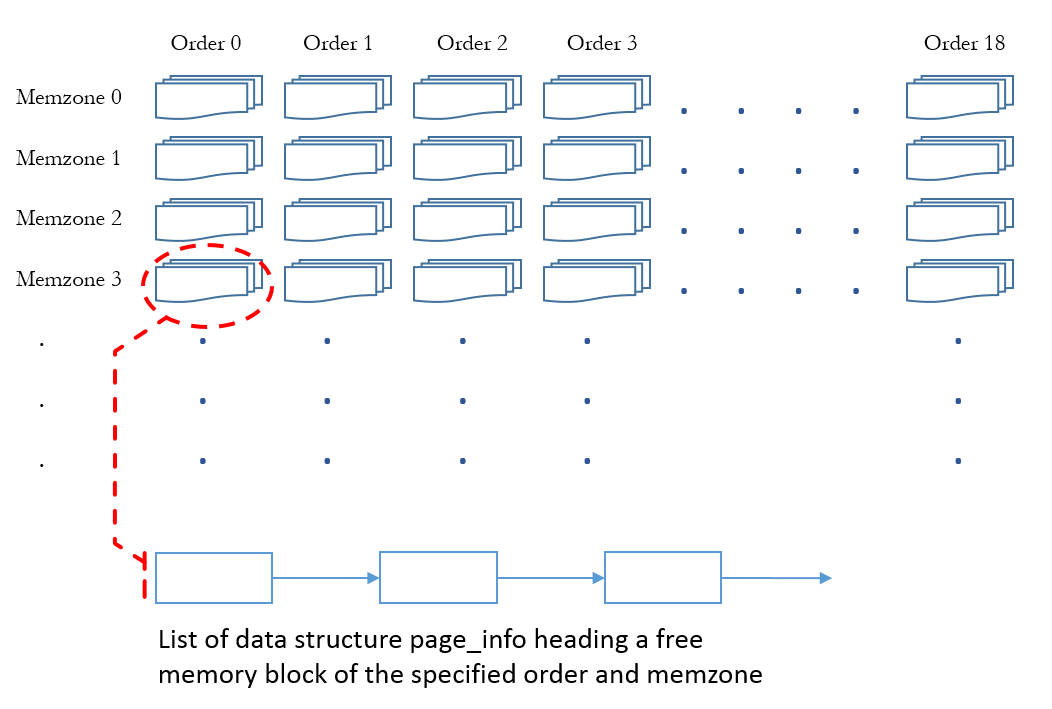
\includegraphics[scale=0.88]{figures/heap_data_structure.png}
\caption{Memory Pool -- \_heap data structure}
\label{fig:heap_struct}
\end{figure}

Each location in the 2-D array contains a list of the pages (actually their corresponding page\_info data structure) representing contiguous memory regions of the corresponding order and memzone. Memory requests are honored at page granularity by alloc\_heap\_pages and its wrapper functions, which extracts contiguous pages from the above \_heap data structure following a buddy system allocation. Pages returned by any domain are added to the memory pool using the free\_heap\_pages function call. This function coalesces any adjacent free regions, if available, and adds the memory pages back to the \_heap data structure. These pages are first scrubbed clean of all information before adding to the pool, protecting the security across domains. The pool is always aggregated to the highest order during these return requests.

Once the memory pool is ready, Domain 0 is given an appropriate amount of memory and the kernel image is copied. The hypervisor follows to build a CPU pool out of the available cores. It initializes VMCS and other associated data structures and hands control over to Domain0 Linux kernel. It is the responsibility of dom0 now to initialize all I/O devices using their appropriate drivers. 

\subsection{Design modifications}

 To enable sharing NVRAM across separate VMs, we have to first recognize it as a memory region. Currently the firmware (BIOS) marks that section with code 90. Due to lack of standardization, this code is subject to change and presently not recognized by Xen. Therefore, the hypervisor treats it as an unrecognized address space. Xen inhibits from either writing to or reading from these addresses.

The first task should be to recognize the memory region, and mark it as Non-Volatile RAM. A separate code word is added to the list of recognized E820 codes, to that effect. After identifying the region, a new NV memory pool is added in the form of an additional data structure \_nvm\_heap. This structure is quite similar to the \_heap data structure explained earlier except that it stores the pages of non-volatile memory. The E820 entries are examined one by one and the appropriate memory pools are populated, i.e. volatile RAM pool (identified by structure \_heap) is filled with RAM pages and non-volatile memory pool (identified by structure \_nvm\_heap) is filled with NVRAM pages.

Separate NVM allocator functions nvm\_alloc\_heap\_pages and nvm\_free\_heap\_pages are defined which operate on the \_nvm\_heap data structure. Similar to the volatile memory management function counterparts, these functions just manipulate the NV memory pool data structure and do not create any additional page table mappings. Since all pages are accessible via direct mapping and Xen does not perform swapping, page table modifications are not needed. The structure, page\_info, is also modified by adding a separate flag to differentiate between volatile and non-volatile pages.

With the above mentioned modifications in place, Xen is able to boot up, identify the available Non-volatile memory and allocate/de-allocate NVRAM pages on demand. A basic non-volatile memory management unit has been setup. It still requires an interface for domains to specify non-volatile memory requirements and request non-volatile memory through the NV MMU. The next section discusses a guest domain creation procedure, where modifications are added to utilize the above infrastructure. 

\section{Guest VM boot procedure}

Booting on bare metal x86 can be quite different from the virtual environment provided by Xen. An x86 CPU starts in 16 bit real mode, with BIOS providing basic essential functions such as hardware information, address space resolution and I/O device drivers. During the boot up procedure, the OS builds page tables and transitions the CPU to protected mode. At this point generally BIOS interrupt calls are unavailable so the OS device drivers are used for I/O. Most of the above functionalities are unavailable in a VM in Xen because the hypervisor boots up first transitioning the machine into protected mode. This poses a problem as the CPU state is totally different in a VM to what an Operating System is expecting.

A guest in Xen can boot in two available modes – PV and HVM. Both of them solve the above issue in separate ways. In PV mode, the OS kernel is modified to allow booting in protected mode. Due to unavailability of BIOS, boot time information is passed to the guest using shared memory pages. There are two types of shared memory pages.

1. Start info page: These pages are mapped to the guest’s address space by Xen. It provides necessary information such as total available memory (essentially the E820 memory map), number of virtual CPUs, console connection, and data structures regarding Xenstore. For boot purposes, Xen explicitly provides only a console device. Any other device must be mapped by the guest kernel using Xenstore services.

2. Shared info pages: A guest kernel needs to explicitly map these pages to its own address space for accessing dynamic runtime information about the virtual machine such as wall clock time, architectural information and event channels. This data is continually updated to reflect the status of the virtual machine.

Information provided through these channels helps in replacing BIOS functionality in PV guests.

HVM mode, on the other hand, is supposed to run unmodified OSes, thus it has to forgo some of the performance benefits of the PV mode and emulate certain devices. Emulation is not optimal because every abstract action is first converted to device specific commands by the guest OS device driver, and these commands are intercepted by Xen. The device emulator reconverts these device specific commands back to the abstract actions that are forwarded to the actual device driver for completion. The Xen split device driver model in PV guests generally runs at a higher level of abstraction avoiding most of the redundant work observed in emulation.

BIOS is emulated by borrowing code from Bochs emulator. It forms the front end in a split device driver model, with the back end handled by code borrowed from QEMU, which is used to emulate devices in HVM mode. Xen starts a domain from the BIOS start point in the virtual 8086 mode present in x86. This mode is actually intended for running legacy application in real mode, alongside protected mode applications. Since it was designed for userspace code, the boot code of an OS (containing a good amount of sensitive instructions) result in numerous traps which have to be handled individually by Xen.

In a hybrid approach, Paravirtualized guests can take the benefit of paravirtualization techniques as well as hardware accelerators while running in HVM mode. The guest can specify a location in its ELF header where the hypercall page can be loaded. It can also execute the CPUID instruction to determine whether it is running on top of Xen or bare metal hardware. If running on Xen, the guest may choose to switch over to Xen specific device drivers, and also map the hypercall page during runtime. However, all these functions are typically performed after the kernel boots up, thus BIOS and QEMU emulator are generally needed during boot-up.

Starting a domain begins with defining a configuration file that includes the disk storage, memory, vCPU and other parameters. The command xl create <filename> performs certain administrative tasks in the userspace domain and then fires up the domain. Initially, the xl tool parses the configuration file to identify resource requirements, most important of them being memory. If sufficient memory is not available, then an attempt is made to free up memory by communicating to Xen the additional memory requirement via Xenstore. This would typically result in Xen inflating the balloon drivers. In the event of still not meeting the memory requirement, the xl tool aborts the domain creation process with an error.

On the other hand, if the memory requirements are met, the tool issues a hypercall (via xend) to build necessary data structures (VMCS and internal Xen data structures) for domain management. The management tool also creates a guest physical address space and sends a hypercall for appropriate memory allocation and page-table mappings. The hypervisor, on receiving this hypercall, allocates pages via the associated functions mentioned in the previous section. It also builds up the hypervisor page tables to map the guest physical pages to actual machine pages. If all is successful then a virtual E820 memory map is created, and the new VM is booted with emulated firmware using code borrowed from Bochs and QEMU.

\subsection{Design modification}
The overall objective of this section is to create an interface for configuration and allocation of Non-volatile memory. Current work focuses on extending this functionality only for HVM guests. Here, implementation details lie in three areas – xl management tool, Bochs emulator, and hypercall structure.

First and foremost, a parameter is added to the configuration file facilitating the specification of the non-volatile memory requirement in Megabytes. This parameter is read by the tool chain, which then creates additional guest physical address space for NVRAM. Actual memory allocation is performed at this point using hypercalls to notify the hypervisor of the guest physical page numbers with emphasis on allocation of contiguous memory blocks to minimize TLB entries. The x86\_64 architecture provides page mapping in the sizes of 1GB, 2MB and 4KB. The allocator moves in descending order for memory requests to satisfy the requirement. A flag is added to the hypercall argument to differentiate between volatile and non-volatile memory requests. If the flag is set, the hypervisor pulls pages out of the NVRAM pool, else it uses the RAM pool for the purpose.

The above procedure completes one of the most critical portions of domain creation. Allocations of both volatile and non-volatile memory are complete and Xen is left with the task of firmware emulation. The toolchain creates virtual E820 table mappings, with an added region to indicate NVRAM with code 90. This completes the boot procedure and the virtual machine is equipped with non-volatile memory. When the VM is turned off, the hypervisor reclaims both RAM and NVRAM pages and adds them to their respective memory pools. 

\include{implementation}


\chapter{\uppercase{Experimental Setup and Results}}


\chapter{\uppercase{Conclusion and Future Work}}

Sharing non-volatile memory in a virtual environment opens up several new challenges and design problems. The main issue is that until now there was no notion of several forms of main memory. Memory was treated as a uniform device, and everything else is left as I/O. NVRAM breaks the conformity, by adding a completely different memory device. Thus it requires a new NV memory management suite, alongside the traditional volatile memory management modules. The two, though share similar jobs and have several contrasting features. It calls  for a modular design of memory management units similar to that present for I/O devices. In a virtual environment, the need is even more important, as memory and I/O are considered as a bottleneck most of the time. Introduction of NVRAM would ease the pressure on I/O disk ops, and memory used as disk cache. 

This work can be considered as a first step in that direction, which brings several interesting research questions. NVRAM has both the properties of disk storage and volatile memory. Thus what direction should it follow while sharing the same, disk or memory? The answer is found in a combination of the two. Since non-volatile memory is a precious resource (like RAM), therefore it cannot be permanently allocated to VMs, like disk space, even when they are not operational. The hypervisor needs to implement a dynamic memory pool which grants NVRAM requests on machine boot up and reclaims them back when the machine is no longer operational. Therefore it also has to follow the same thin provisioning schemes as main memory, implementing a balloon driver to retrieve memory back.  

All these memory like operations brings us to the main difference between volatile and non-volatile memory. In one case, where volatile data ceases to exist as soon as the machines are powered off, non-volatile RAM on the other hand preserves data. This data needs to be preserved between a reboot cycle for a VM. The same needs to follow for entire system (including the hypervisor) reboots too. While data retention during entire system reboots is taken care of in hardware, mapping of non-volatile resources should also be maintained. The task again can be broken down into two separate simpler subtasks.  

1. Preserve the non-volatile data for VMs even after the VM is powered off. 

2. Maintain the hypervisor page table mappings across system reboot. 

When a VM is created, its non-volatile data needs to be restored to its state before power down. Additionally, during power off procedure, NVRAM pages need to be reclaimed, as it is a critical resource. Thus the data has to be shipped to disk. The above requirement is very similar to the “save state” and “restore state” features offered for virtual machines. Here all the data present in main memory is written to a file on disk. The memory state is restored from a file on disk, during the restore procedure. The same procedure can be followed for NVRAM region thereby not wasting memory when the VM is non-operational. The file location can be provided in the VM configuration file. 

Since memory does not expect presence of any valid data during the boot procedure, the available memory regions are usually initialized from scratch. The same procedure is followed for the current implementation of NVRAM memory initialization in the hypervisor. Although we still retain persistent data, the respective mappings of memory pages are lost. It is very important to emphasize again that non-volatile memory proves superior to volatile memory only during unplanned power failures. For all other cases there is no advantage of NVRAM over RAM except for faster boot up times. During a planned reboot cycle, volatile RAM regions can also preserve data by saving the state on disk during shutdown and restoring it on start up. Many operating systems provide a similar feature called as hibernate. Therefore the main task at hand is to restore the system state in NVRAM after start up, if power is lost at a random point in runtime. 

This issue is not completely new, and filesystems have solved a significant part of the problem. A separate NVRAM area can be set aside by the hypervisor for maintaining metadata structures. On system boot up, the NV memory manager would need to read the metadata and recreate the NVRAM memory mappings present before the system was powered off. This state restoration should incorporate page allocations and hypervisor page table mappings of all virtual machines, along with their data, because the system needs to guarantee data persistence for power failures during random runtime conditions. It can be troublesome because just after power up, a VM does not have any existence except its config file and disk space, while the NVRAM area still remains active.  

One possible solution is to divide NVRAM metadata section in several sections, with each running VM occupying one section. The hypervisor is also provided with a separate section for storing its relevant data structures. The VMs store their hypervisor page tables in this metadata section along with the location of a file where the contents are to be paged out, if the VM is turned off. The file location can be specified and passed through the config file associated with that domain. Xen, in its metadata section can store all the data structures pertaining to the non-volatile memory management unit, such as page\_struct, \_nvm\_heap, etc. During the startup process the hypervisor would read the metadata to determine the state of NVRAM and the amount of free memory available in the NV memory pool. Therefore, instead of rebuilding the data structures, Xen would just need to update the associated memory pointers. In the event of an improper system shutdown, several VMs might not have exited properly and could still be occupying the allocated non-volatile memory. As a part of boot up operations, the hypervisor can page out those NVRAM regions to the associated files on disk to free up redundant space and restore the system state.

\include{conclusion}

%fix spacing in bibliography, if any...
%%%%%%%%%%%%%%%%%%%%%%%%%%%%%%%%%%%%%%%%%%%%%%%%%%%%%%%%%%%%%
\let\oldbibitem\bibitem
\renewcommand{\bibitem}{\setlength{\itemsep}{0pt}\oldbibitem}
%%%%%%%%%%%%%%%%%%%%%%%%%%%%%%%%%%%%%%%%%%%%%%%%%%%%%%%%%%%%%%%
%%%%%%%%%%%%%%%%%%%%%%%%%%%%%%%%%%%%%%%%%%%%%%%%%%%
%
%  New template code for TAMU Theses and Dissertations starting Fall 2012.  
%  For more info about this template or the 
%  TAMU LaTeX User's Group, see http://www.howdy.me/.
%
%  Author: Wendy Lynn Turner 
%	 Version 1.0 
%  Last updated 8/5/2012
%
%%%%%%%%%%%%%%%%%%%%%%%%%%%%%%%%%%%%%%%%%%%%%%%%%%%


%%%%%%%%%%%%%%%%%%%%%%%%%%%%%%%%%%%%%%%%%%%%%%%%%%%%%%%%%%%%%%%%%%%%%%
%%                           REFERENCES 
%%%%%%%%%%%%%%%%%%%%%%%%%%%%%%%%%%%%%%%%%%%%%%%%%%%%%%%%%%%%%%%%%%%%%

\phantomsection
\addcontentsline{toc}{chapter}{REFERENCES}

\renewcommand{\bibname}{{\normalsize\rm REFERENCES}}

\bibliographystyle{plain}
\bibliography{references}
% \include{appendices}


\end{document}
